% MD5 ("frastoca") = d4e02542ff15febf3ca60b1e048d23db
%
%  untitled
%
%  Created by Andrés Alessandro León Baldelli.
%  Copyright (c) 2015  All rights reserved.
%
\documentclass[]{article}

% Use utf-8 encoding for foreign characters
\usepackage[utf8]{inputenc}
\usepackage{pmboxdraw}

\usepackage[lined]{algorithm2e}
\usepackage[top=1cm, left=1.5cm, right=1.5cm, bottom=1cm]{geometry}
% pygments
\usepackage{fancyvrb}
\usepackage{color}
\usepackage[english]{babel}
\usepackage{datetime}
% end pygments
\usepackage{geometry}
\usepackage{eurosym}
\usepackage[backend=biber,style=numeric,natbib=true,giveninits=true,url=false,doi=false,isbn=false,maxnames=5]{biblatex}
% \addbibresource{biblio.bib}
%\AtEveryBibitem{  \clearfield{day}  \clearfield{month}  \clearfield{endday}  \clearfield{endmonth}}

\usepackage[pdftex,pdfauthor={Andres A Leon Baldelli},pdftitle={},pdfsubject={},pdfkeywords={},pdfproducer={Latex with hyperref},pdfcreator={pdflatex}]{hyperref}
\usepackage{import}

% Running Headers and footers
%\usepackage{fancyhdr}

% Multipart figures
%\usepackage{subfigure}
% More symbols
\usepackage{amsmath}
\usepackage{amssymb}
\usepackage{latexsym}
\usepackage{multicol}

% Surround parts of graphics with box
\usepackage{boxedminipage}
% Package for including code in the document
\usepackage{listings}

% If you want to generate a toc for each chapter (use with book)
\usepackage{minitoc}

% This is now the recommended way for checking for PDFLaTeX:
\usepackage{ifpdf}

% 
\newenvironment{system}% 
{\left\lbrace\begin{array}{@{}l@{}}}% 
{\end{array}\right.} 

\usepackage[shortlabels,inline]{enumitem}
\setlist[itemize,1]{label={\textbullet}}
\setlist{noitemsep}
\setlist[1]{labelindent=\parindent,
  itemsep=0ex,
  leftmargin=1em,
  labelwidth=10em
  }
\setlist*[enumerate,1]{%
  label=(\roman*),
}
\newlist{inlinelist}{itemize*}{1}
\setlist[inlinelist,1]{%
  label={},
  before=\unskip{: }, itemjoin={{; }}, itemjoin*={{ et }}
}
\newcommand{\proj}{\emph{FUCK HSBC}}
\input{/Users/kumiori/Documents/WIP/tex_macros/incl_macro_gen.tex}
\ifpdf
\usepackage{graphicx}
% \fi
\title{
\vspace{-2em}
\textbf{``Class Stability'' 50/50} - 
Project: \textbf{\proj}~  }
\author{  
\emph{ALB}\footnote{}~,
}

\date{\vspace{-5em}}

\begin{document}

\ifpdf
\DeclareGraphicsExtensions{.pdf, .jpg, .tif}
\else
\DeclareGraphicsExtensions{.eps, .jpg}
\fi

\maketitle


\begin{center}
\Large{}






\end{center}

\noindent\emph{\textbf{Keywords:} 
}

\medskip

\textbf{Abstract}
% Fuck HSBC, and the banking system \emph{as a consequence}.
\section{Context}
With help from the automated language \emph{graph transversal} ride. A fast one:
we analyse a few classes of damage models, for fun and !profit.



\begin{figure}[htbp]
  \centering
  \includegraphics[width=.8\textwidth]{../figures/generic_class_analyser.png}
  \caption{class analysis}
  \label{fig:class-analyser}
\end{figure}

\section*{ATk = LS = JJK}
\newcommand{\ilen}{\ell}
\newcommand{\sigmac}{\sigma_c}

State = $y:=(u, \alpha)$
Material parameters:
{k: k, E0: 1, w1: w1, $\ilen$: $\ilen$, L: L} are variables.

\textbf{General class (without material parameters)}
\subimport{../../playground/nb/}{/model-atk.txt}
\textbf{With material parameters}
\subimport{../../playground/nb/}{/model-atk-matpar.txt}

\begin{verbatim}
  atk = DefaultDamage(state, _matpar)


ana = ModelAnalysis(atk)
_crit = sp.diff(atk.energy(state), a).subs({u: _u0, a: _a0}).simplify()
_crit
\end{verbatim}


$$
0=- \frac{0.5 E_{0} k t^{2}}{L^{2} \left(k \alpha{\left(x \right)} - \alpha{\left(x \right)} + 1\right)^{2}} + w_{1}
$$

critical load

$$
0=- \frac{0.5 E_{0} k t^{2}}{L^{2}} + w_{1}
$$

\begin{equation}
  \label{eqn:mod-crit}
  % \left\{
    u{\left(x \right)} = \frac{t x}{L} \qquad
  \alpha{\left(x \right)} = 
  \begin{cases} 
      -- \frac{t}{L \sqrt{w_{1}}} & \text{for}: t \geq \\ 
      0 & \text{otherwise}
  \end{cases}
  % \right\}
\end{equation}


\begin{figure}[htbp]
  \centering
  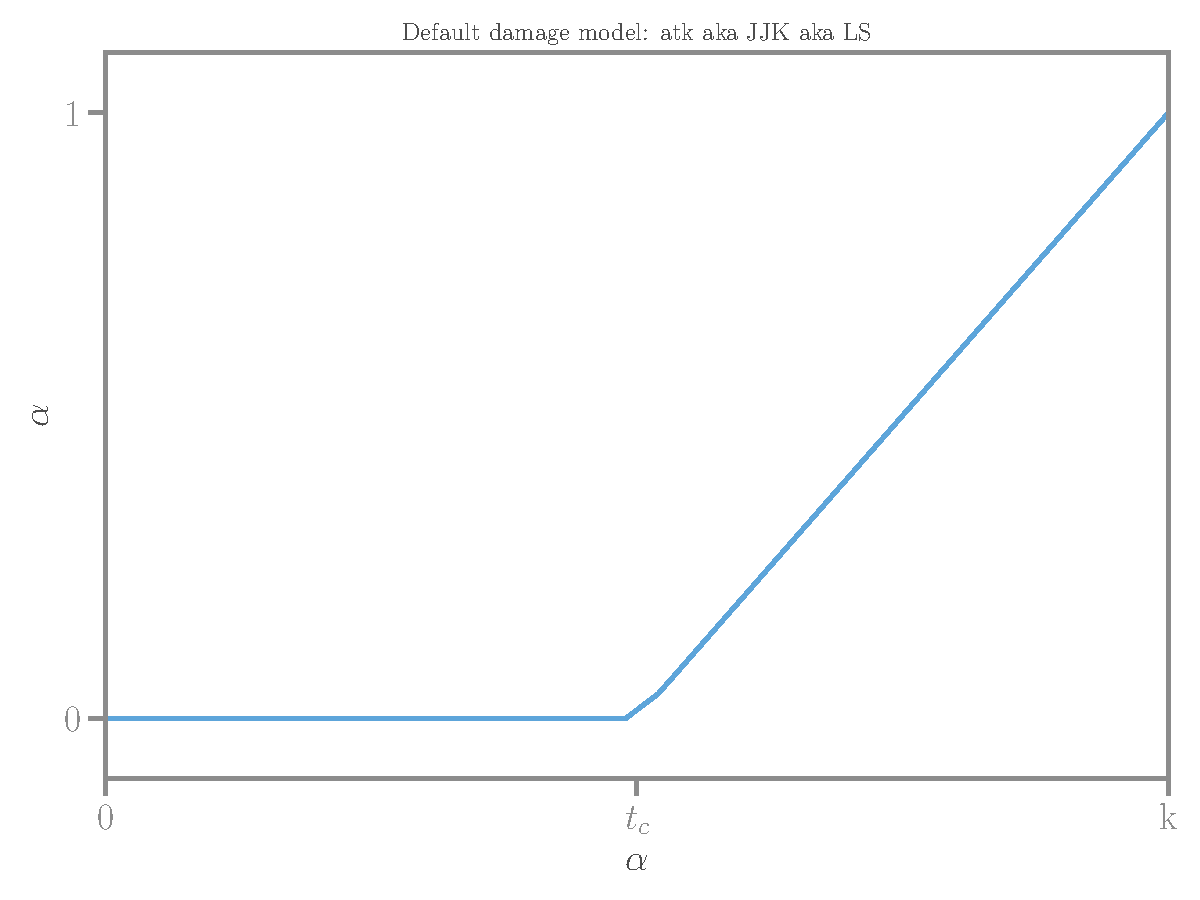
\includegraphics[width=.33\textheight]{../figures/atk-alpha-homog.pdf}
  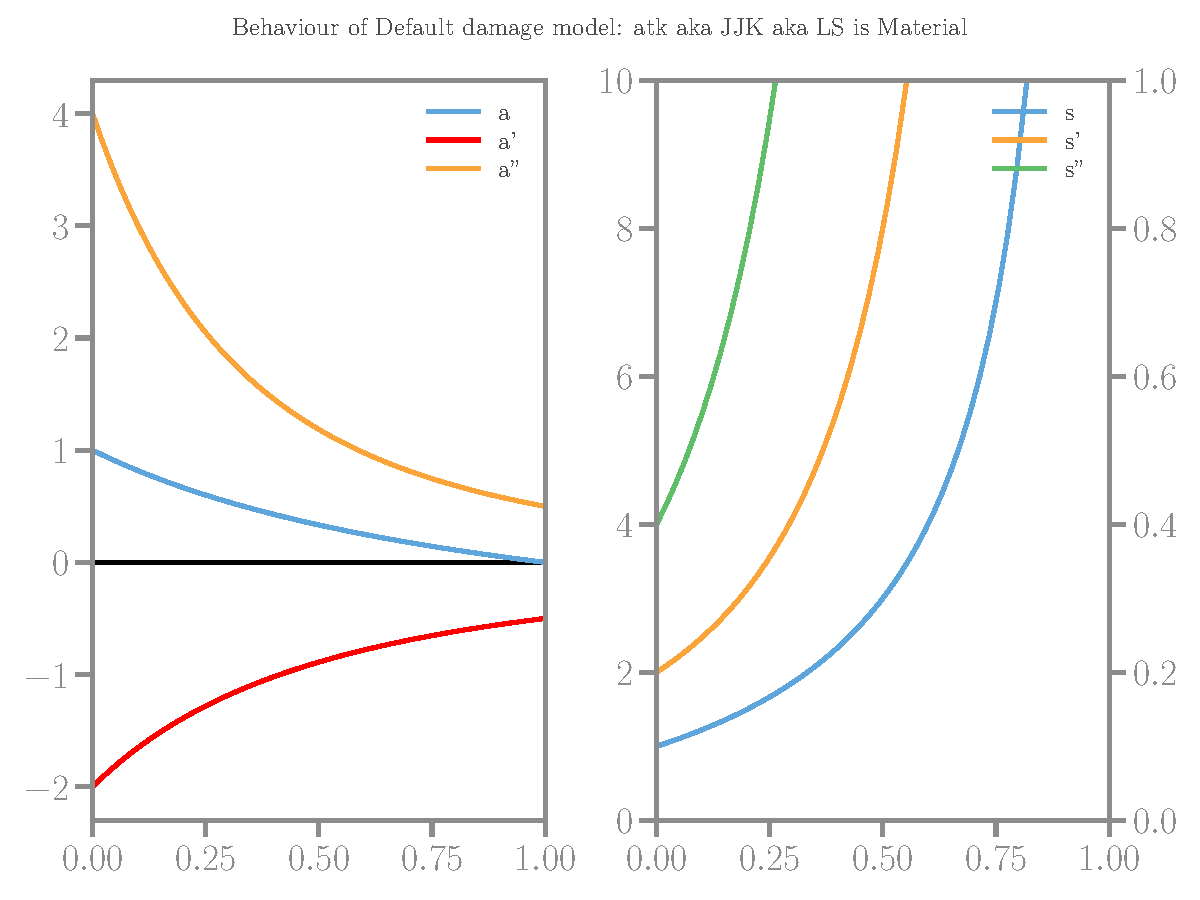
\includegraphics[width=.33\textheight]{../figures/atk-model.pdf}
  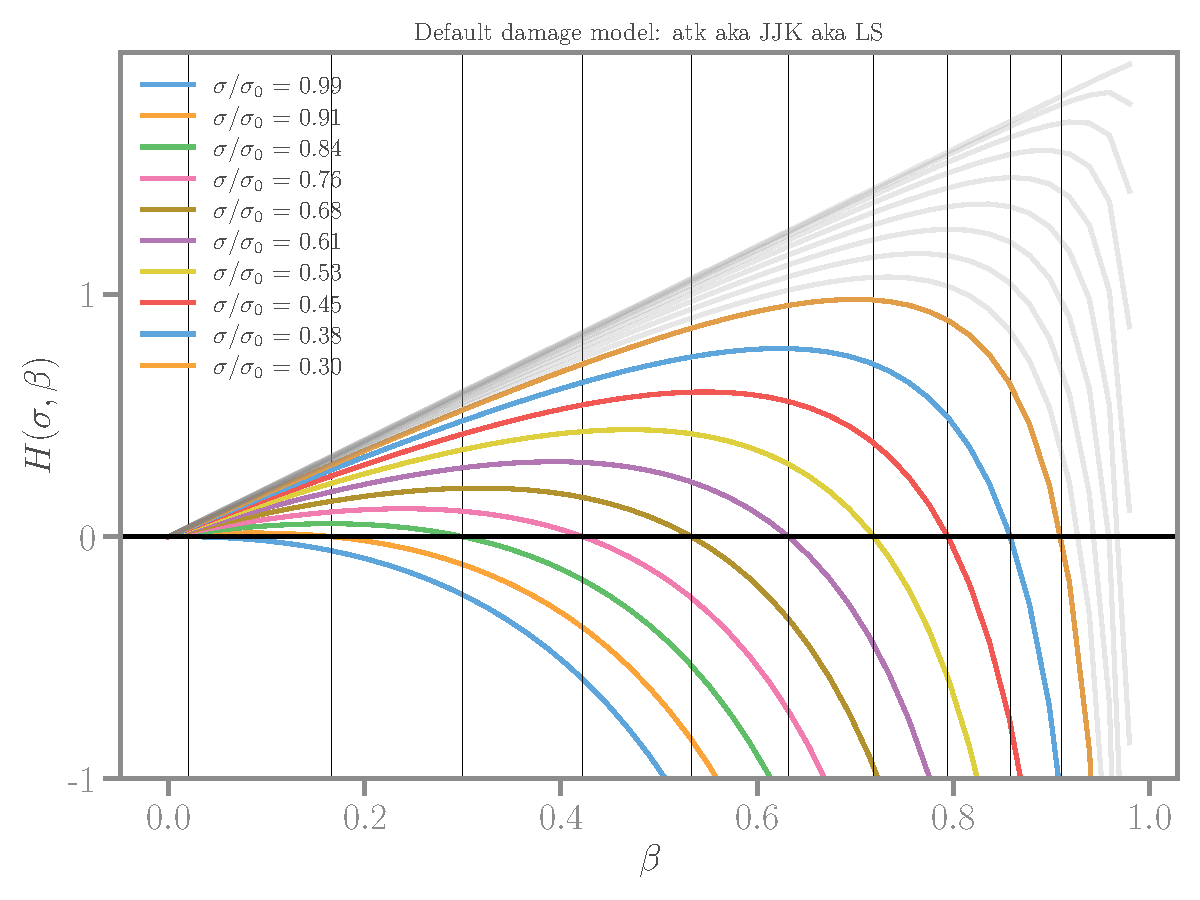
\includegraphics[width=.33\textheight]{../figures/atk-Hbeta.pdf}
  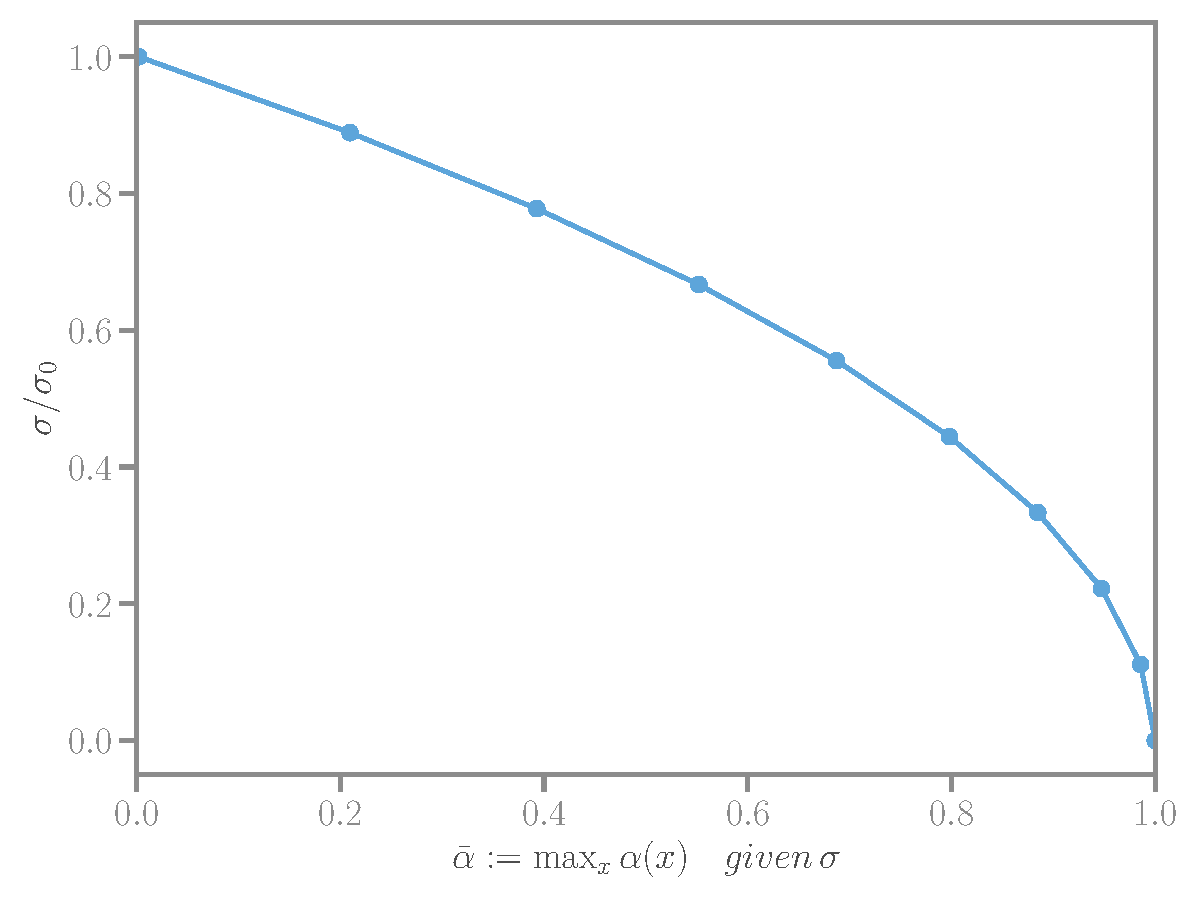
\includegraphics[width=.33\textheight]{../figures/atk-maxalpha.pdf}
  \caption{class analysis}
  \label{fig:class-analyser}
\end{figure}





Homogeneous response

\begin{equation}
  \label{eqn:mod-homog}
  \begin{cases}
    \frac{- L w_{1} + 0.707106781186548 t \sqrt{E_{0} k w_{1}}}{L w_{1} \left(k - 1.0\right)} & \text{for} : t \geq 1.4142135623731 L \sqrt{\frac{w_{1}}{E_{0} k}} \\ 
    0 & \text{otherwise} 
  \end{cases}
\end{equation}






\section*{ATn}
\subsection*{$n=1$}

\textbf{General class (without material parameters)}
\subimport{../../playground/nb/}{/model-at1.txt}
\textbf{With material parameters}
\subimport{../../playground/nb/}{/model-at1-matpar.txt}



\subsection*{$n=2$}


matpar = ${n: 1, E0: 1, w1: 1, \ilen: \ilen}$



\begin{Verbatim}
  ana.criterion(), ana.critical_load(), ana._homogeneous_alpha()  
\end{Verbatim}



\begin{equation}
  \label{eqn:mod-criterion}
  0=- \frac{1.0 E_{0} t^{2}}{L^{2}} + 1
\end{equation}

critical load $t_c = L \sqrt{\frac{1}{E_{0}}}$

\begin{equation}
  \label{eqn:mod-energy}
E(y)  =  \int_0^L
\ilen^{2} \left(\frac{d}{d x} \alpha{\left(x \right)}\right)^{2} + \frac{1}{2} E_0\left(1 - \alpha{\left(x \right)}\right)^{2} \left(\frac{d}{d x} u{\left(x \right)}\right)^{2} + \alpha{\left(x \right)}
\end{equation}


homogeneous state

\begin{equation}
  \label{eqn:mod-homogeneous}
  \alpha_t =
  \begin{cases}
    1 - \frac{L^{2}}{E_{0} t^{2}} & \text{for}\: t \geq 1 \\
    0 & \text{otherwise} \end{cases}
\end{equation}



\begin{figure}[htbp]
  \centering
  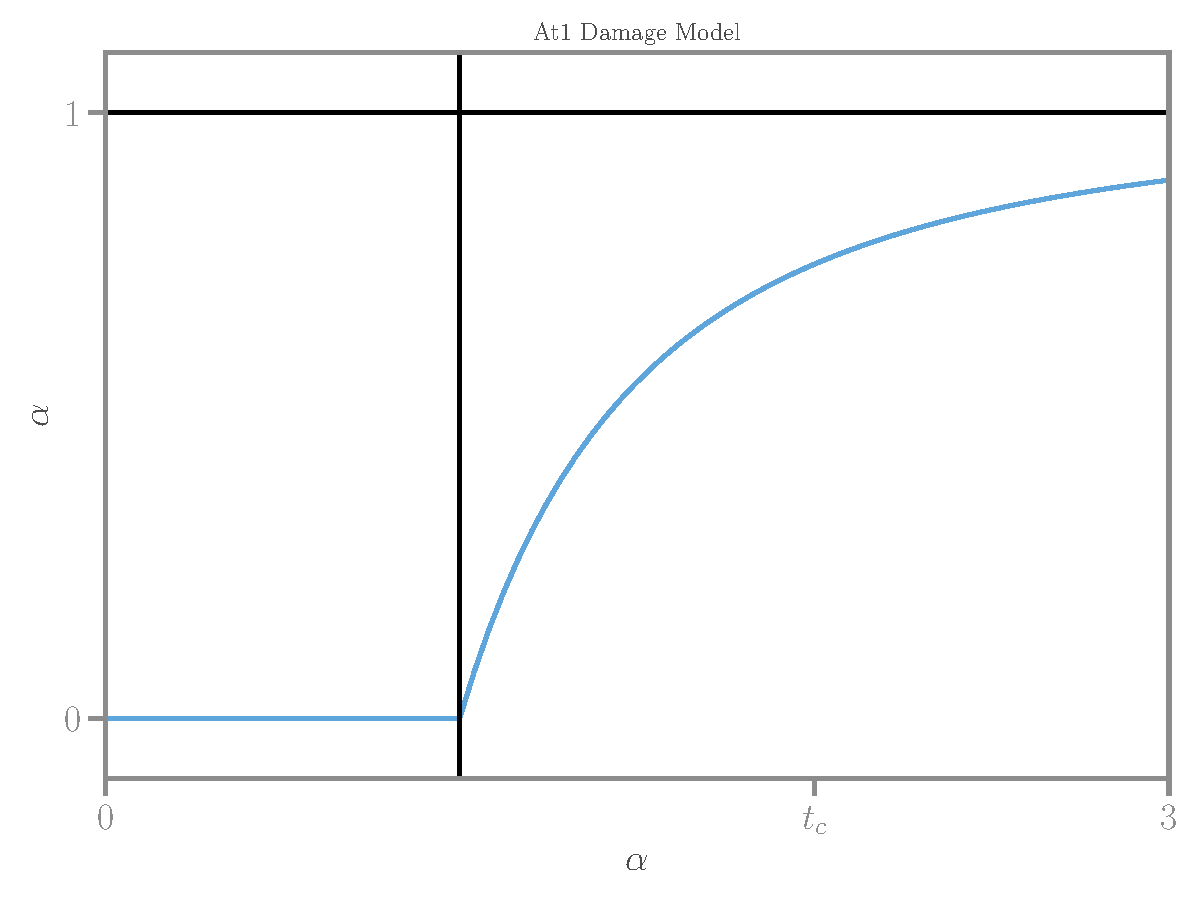
\includegraphics[width=.33\textheight]{../figures/at1-alpha-homog.pdf}
  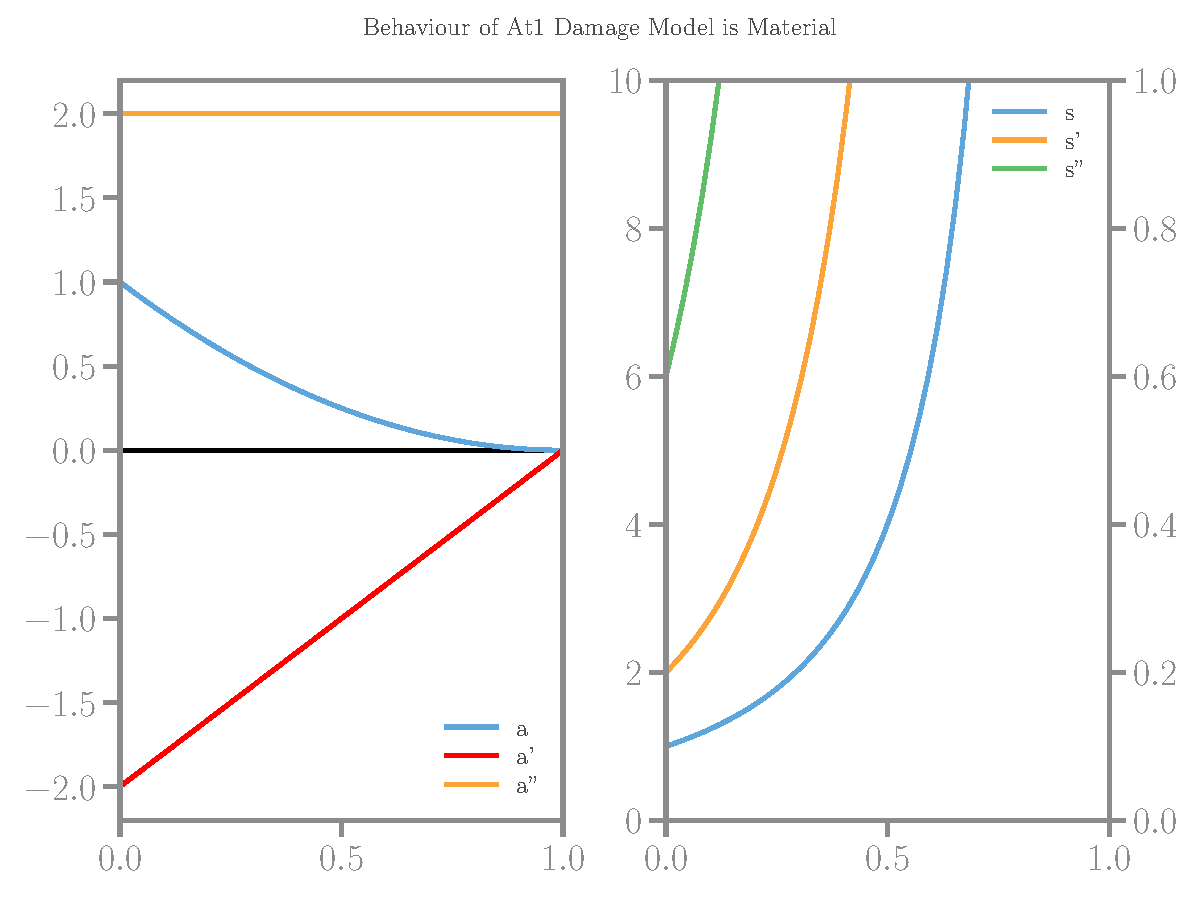
\includegraphics[width=.33\textheight]{../figures/at1-model.pdf}
  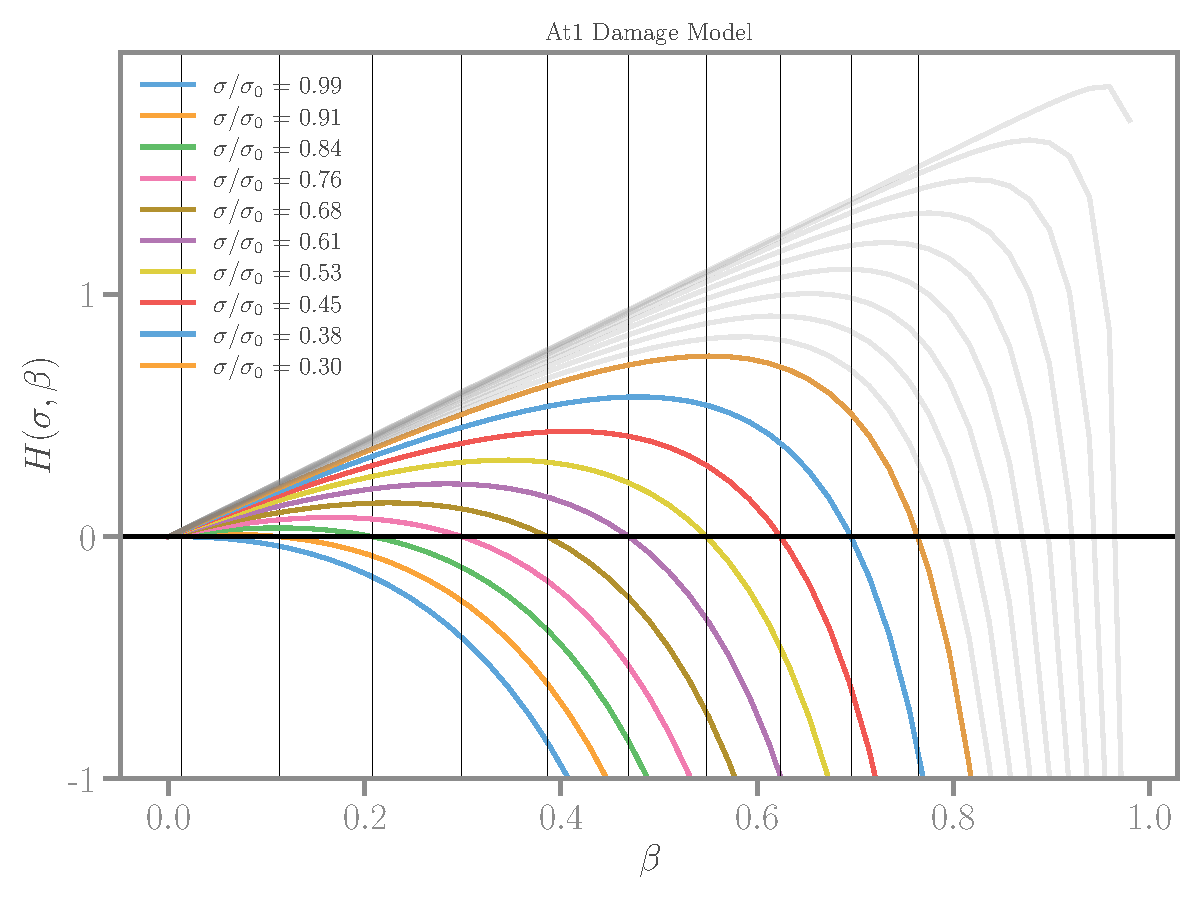
\includegraphics[width=.33\textheight]{../figures/at1-Hbeta.pdf}
  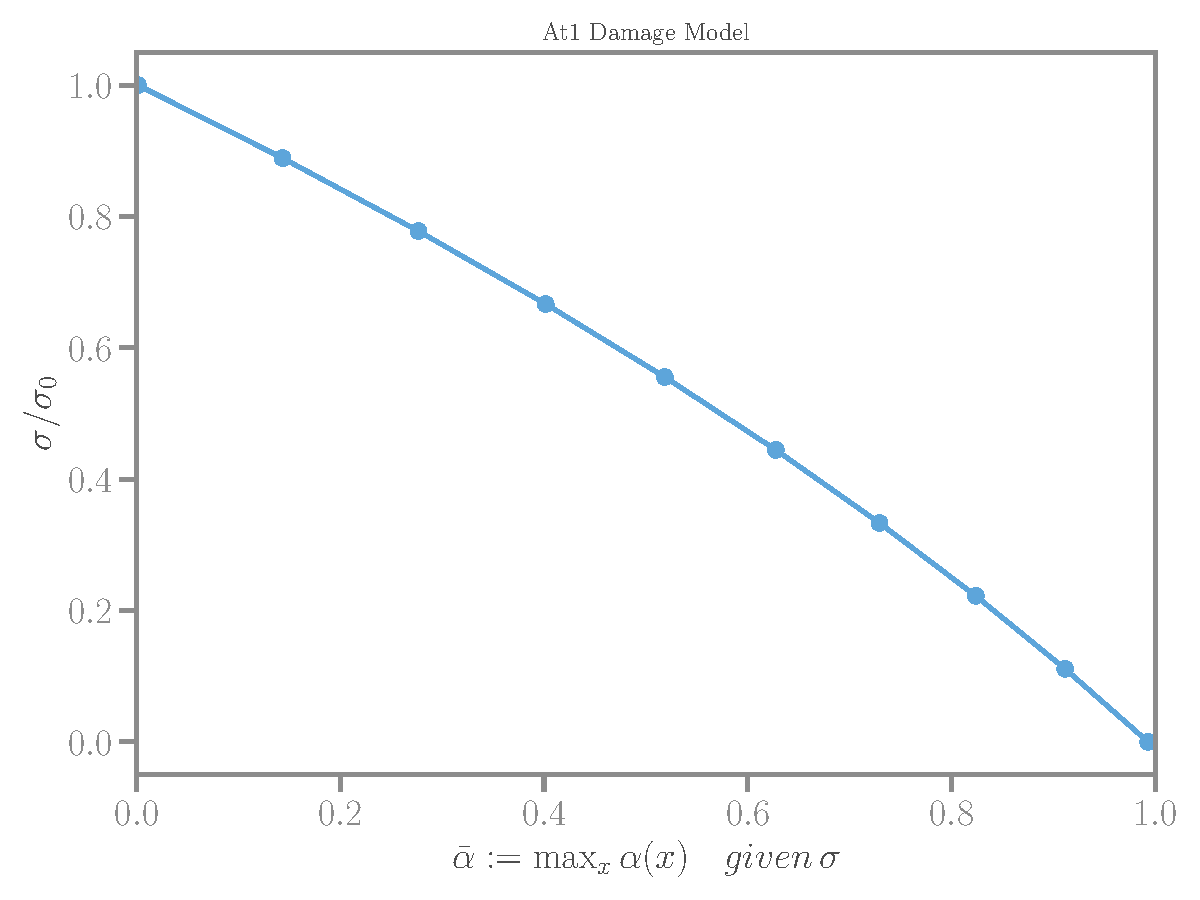
\includegraphics[width=.33\textheight]{../figures/at1-maxalpha.pdf}
  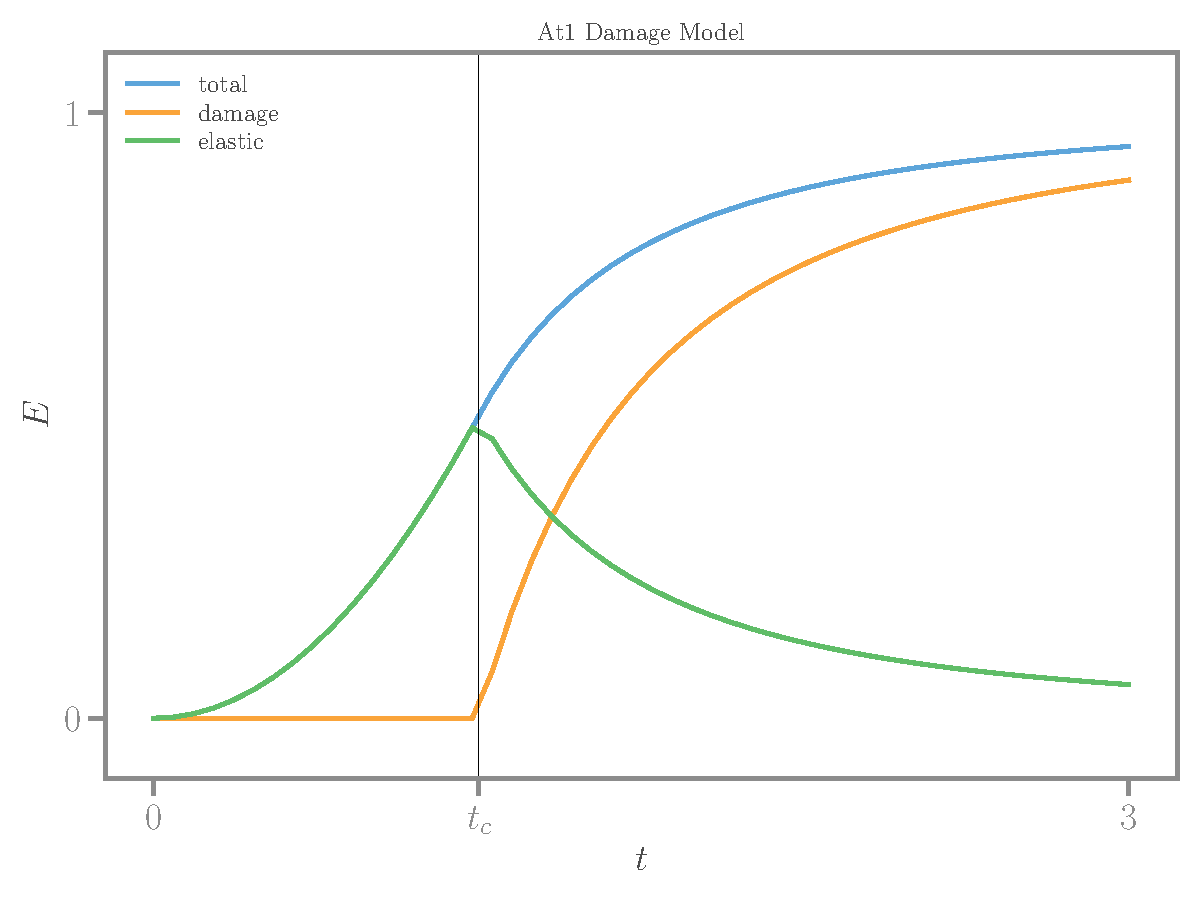
\includegraphics[width=.33\textheight]{../figures/at1-energies-homog.pdf}
  \caption{class analysis}
  \label{fig:class-analyser}
\end{figure}

\section*{PQ}


\textbf{General class (without material parameters)}
\subimport{../../playground/nb/}{/model-pq.txt}
\textbf{With material parameters}
\subimport{../../playground/nb/}{/model-pq-matpar.txt}


energy
\begin{equation}
  \label{eqn:mod-energy}
E(y)  =  \int_0^L
0.5 E_{0} \left(1 - \alpha{\left(x \right)}\right)^{q} \left(\alpha{\left(x \right)} + 1\right)^{- p} \left(\frac{d}{d x} u{\left(x \right)}\right)^{2} + w_{1} \left(\ilen^{2} \left(\frac{d}{d x} \alpha{\left(x \right)}\right)^{2} + \frac{\sigma_c^{2} \left(p + q\right) \alpha{\left(x \right)}}{E_{0}}\right)\end{equation}


parameters
$p, q, E_0, L, w_1, \ilen, \sigma_c $

criterion
\begin{equation}
  \label{eqn:mod-criterion}
  0=
\left(p + q\right) \left(- \frac{ E_{0}^{2} t^{2}}{2L^{2}} + w_{1} \sigma_c^{2}\right)
\end{equation}



\begin{figure}[htbp]
  \centering
  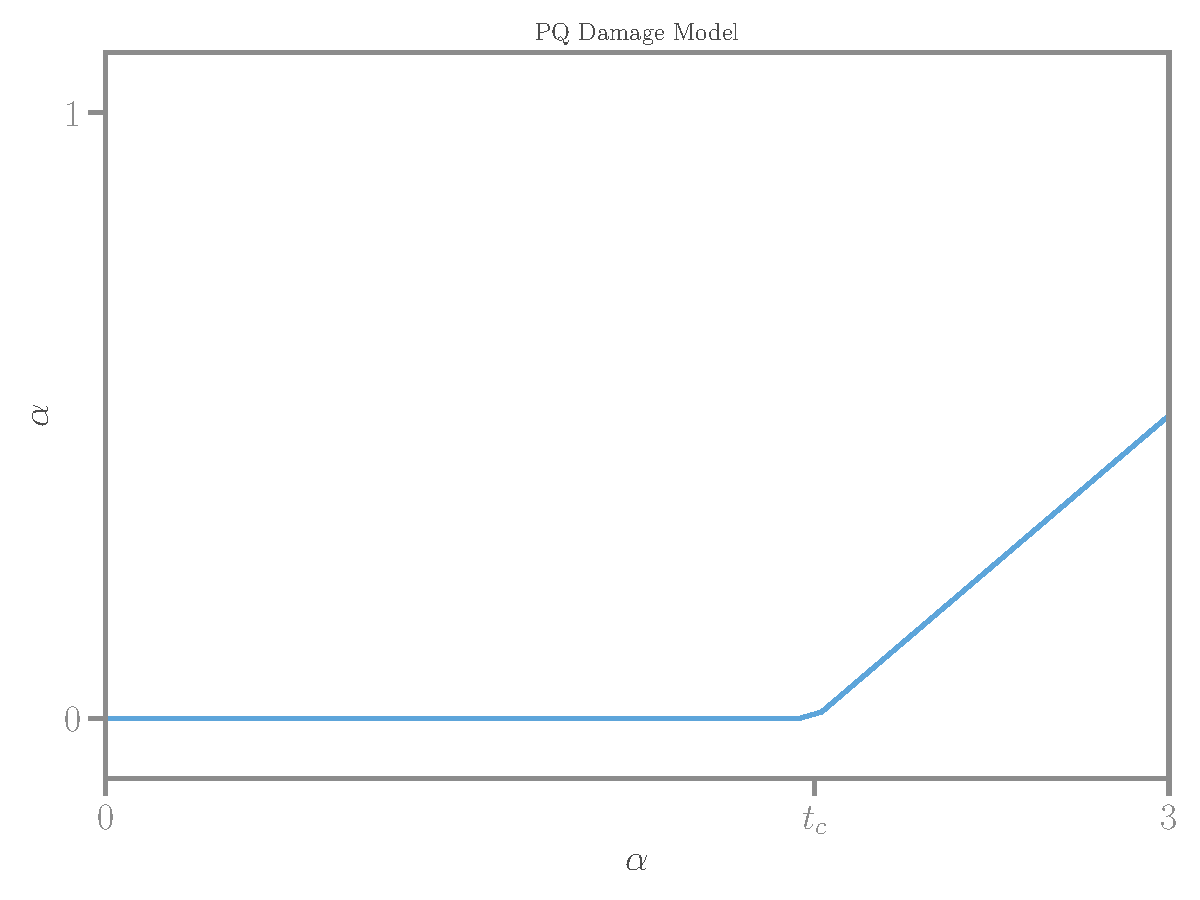
\includegraphics[width=.33\textheight]{../figures/pq-alpha-homog.pdf}
  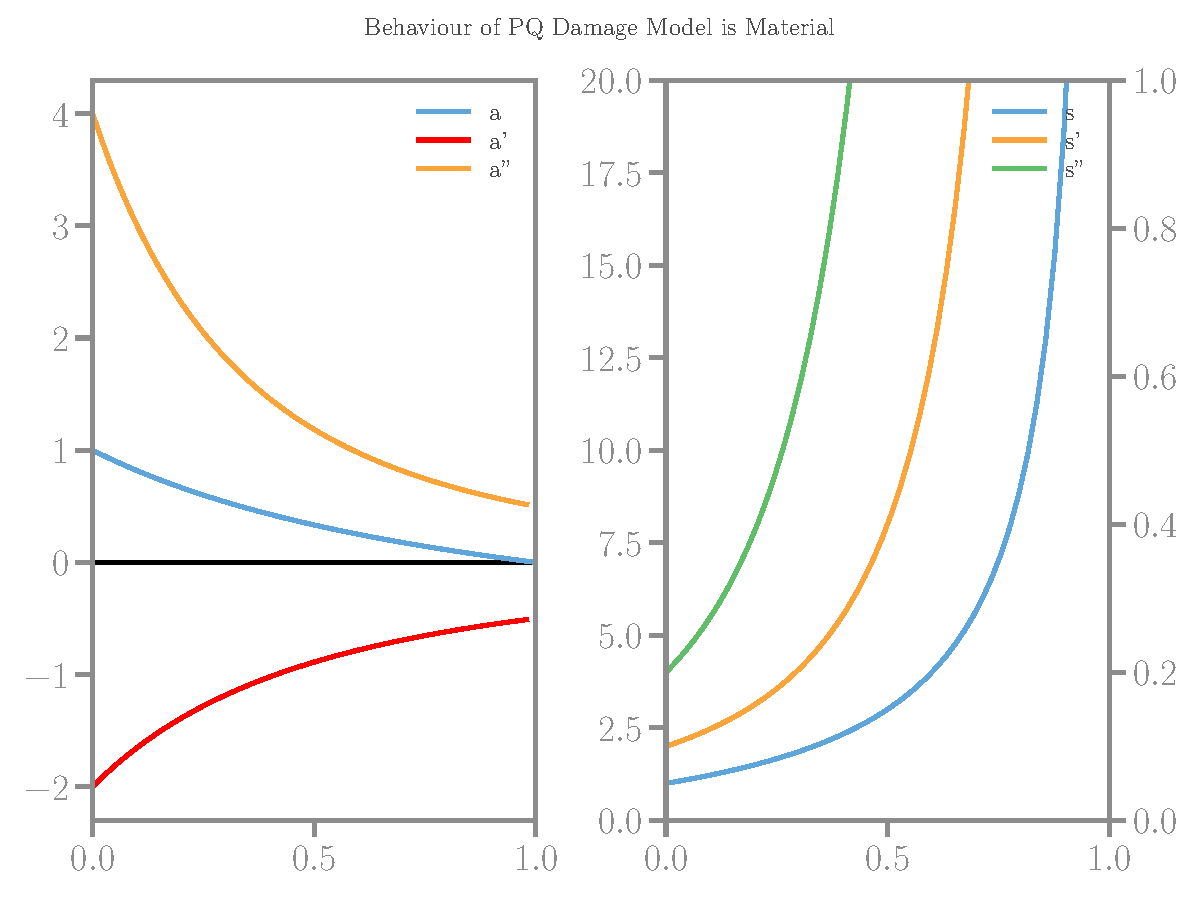
\includegraphics[width=.33\textheight]{../figures/pq-11-model.pdf}
  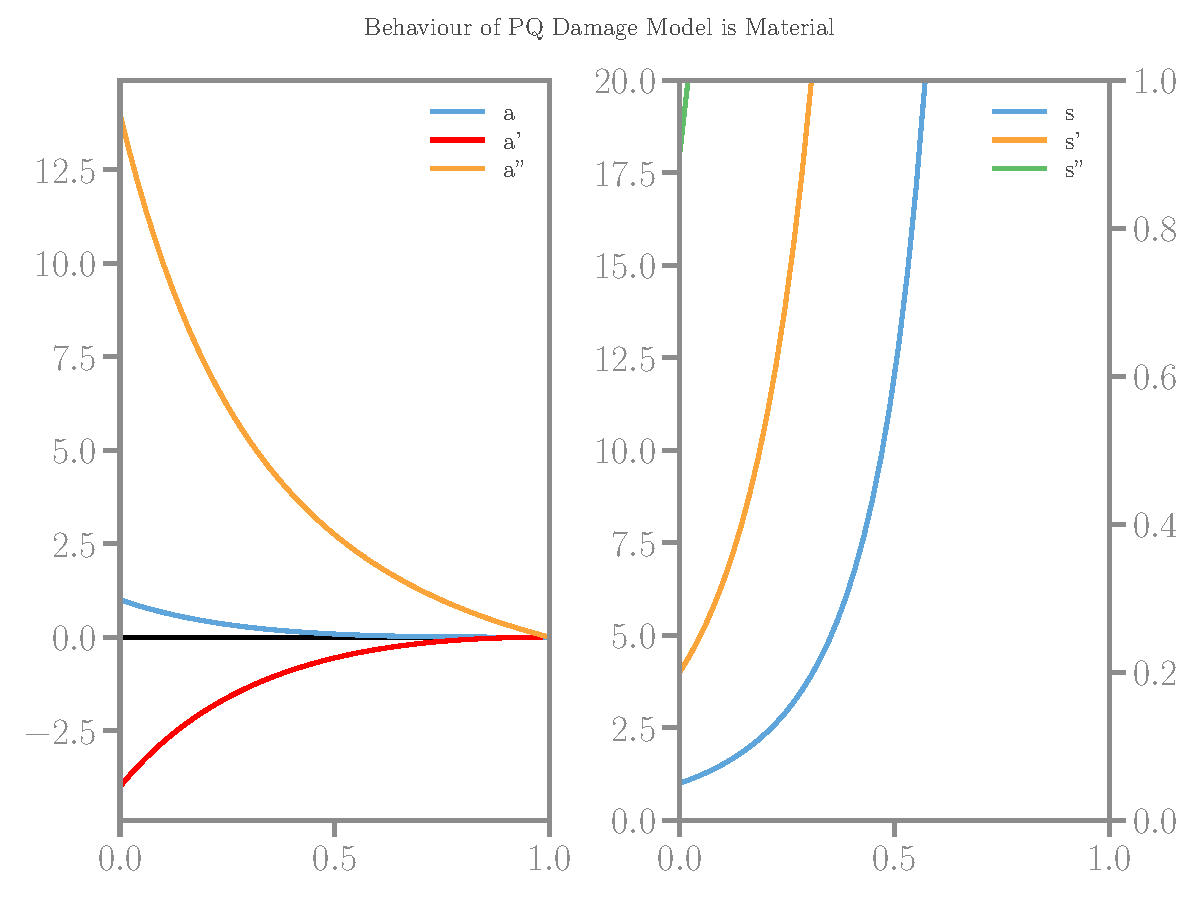
\includegraphics[width=.33\textheight]{../figures/pq-13-model.pdf}
  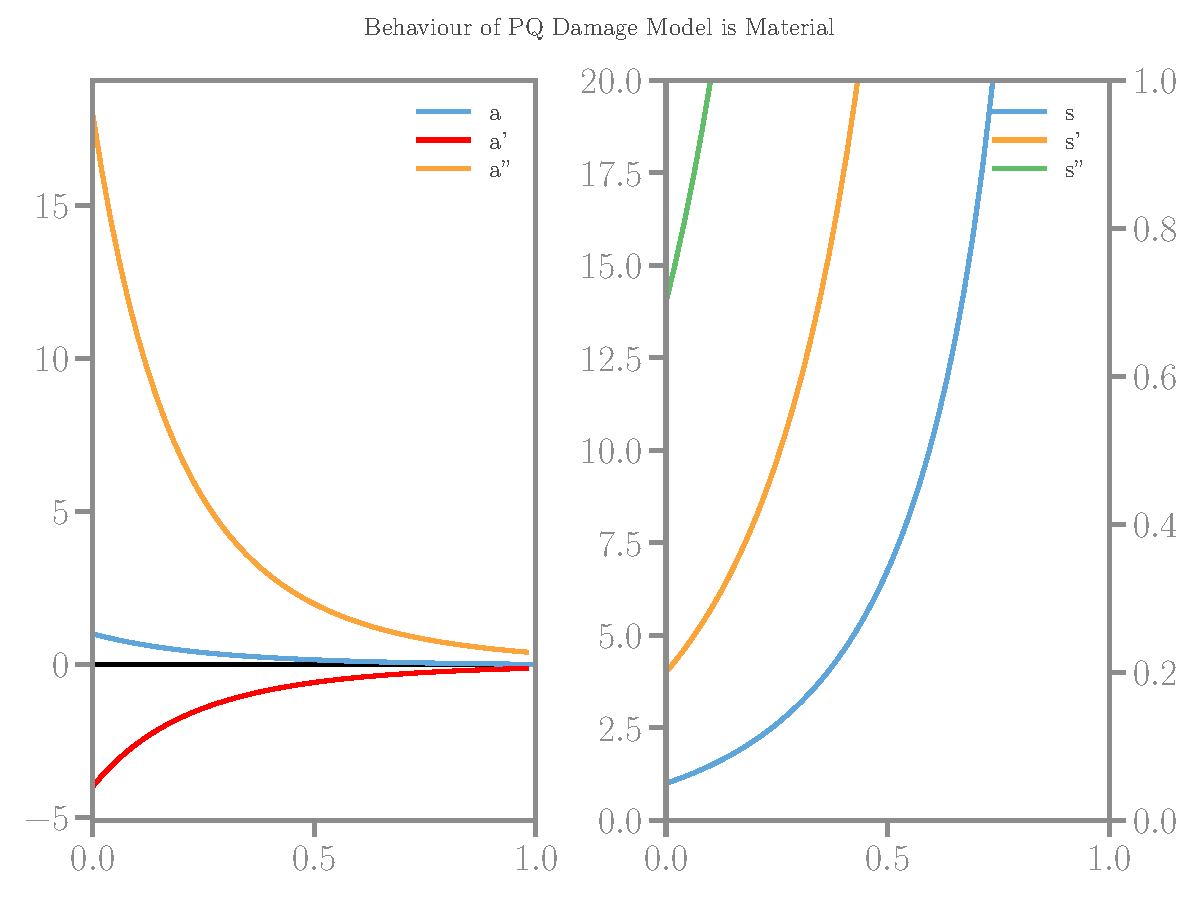
\includegraphics[width=.33\textheight]{../figures/pq-31-model.pdf}
  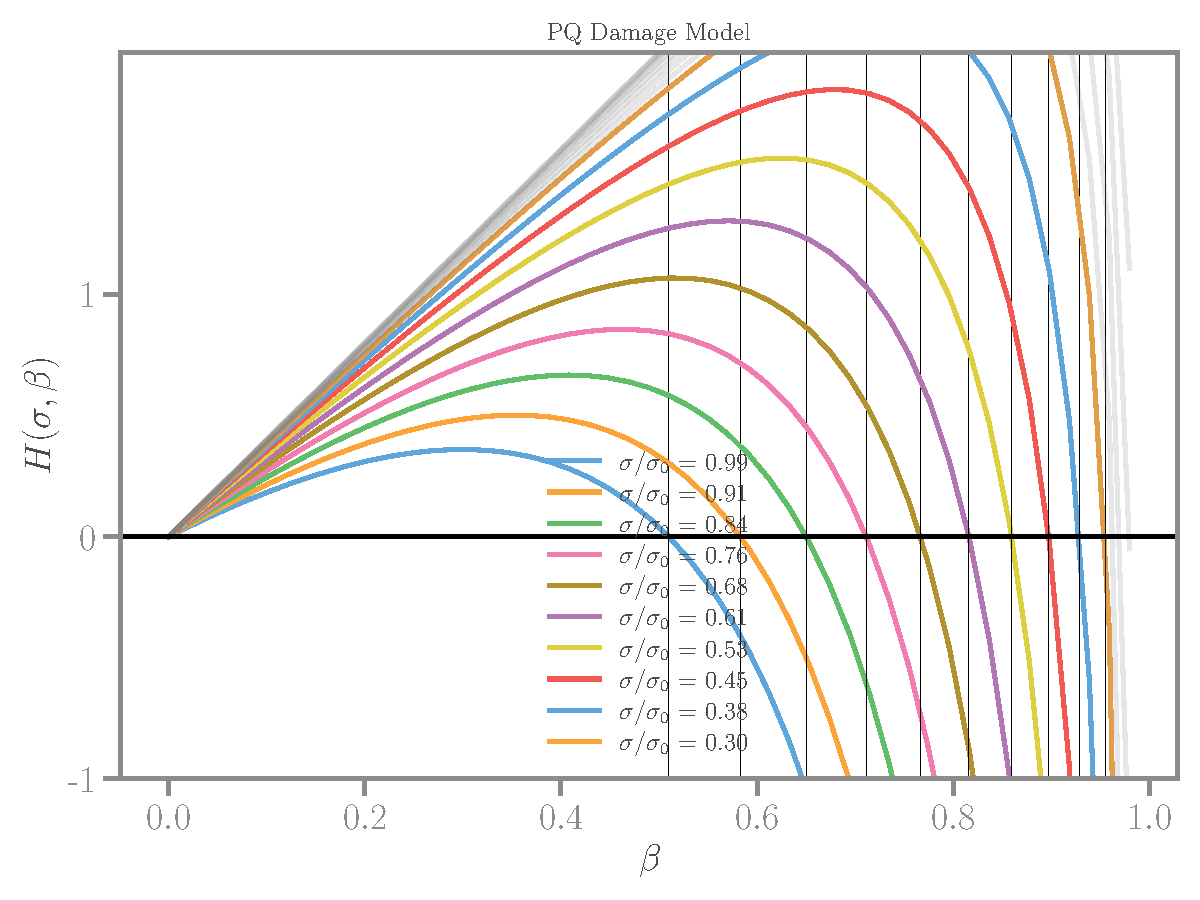
\includegraphics[width=.33\textheight]{../figures/pq-Hbeta.pdf}
  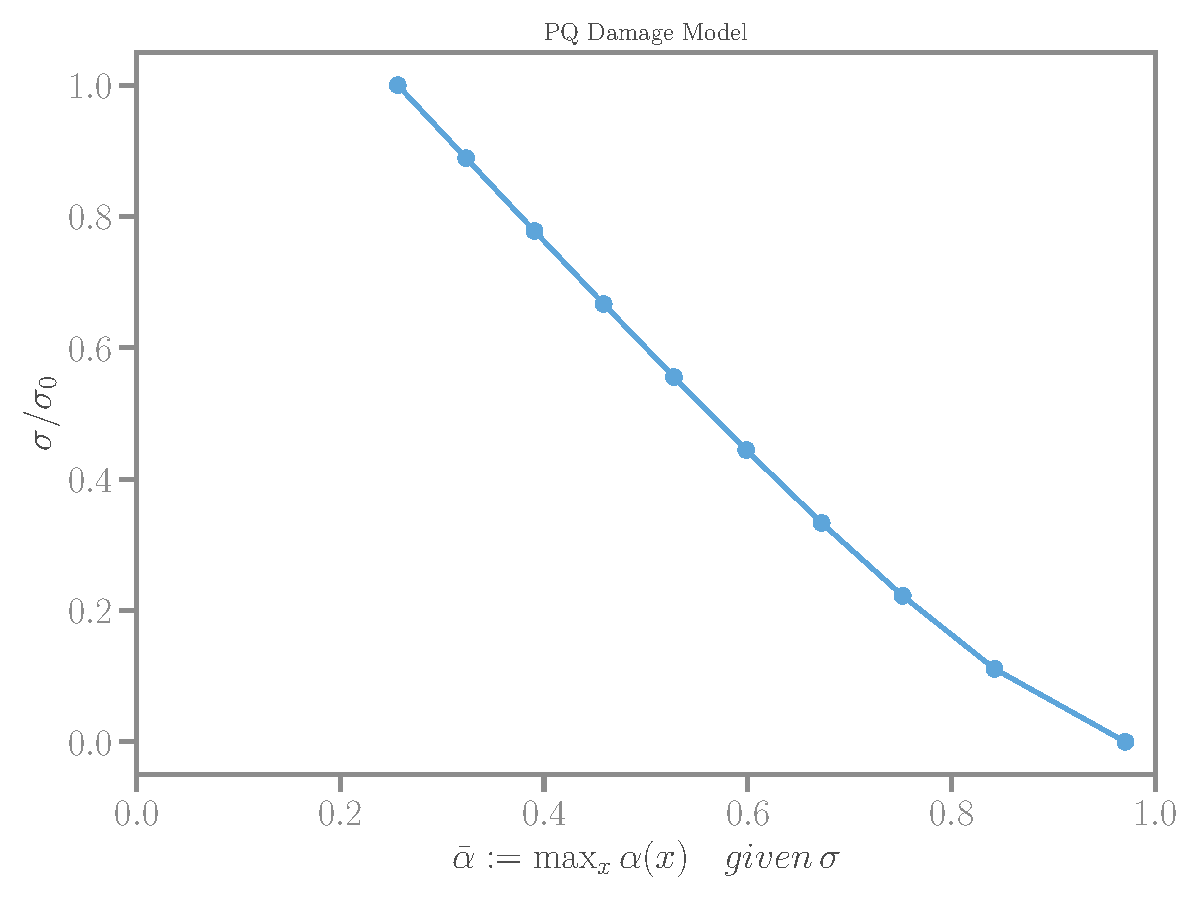
\includegraphics[width=.33\textheight]{../figures/pq-maxalpha.pdf}
  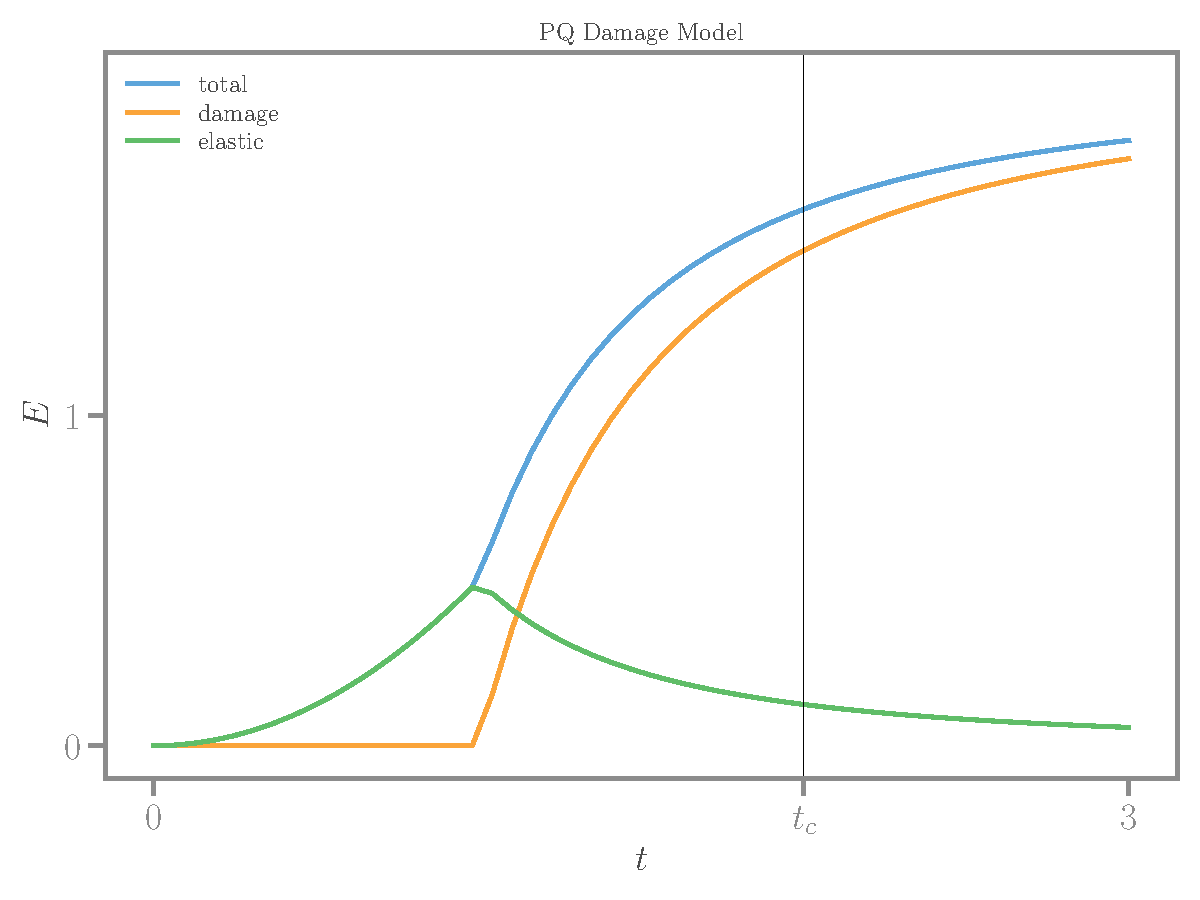
\includegraphics[width=.33\textheight]{../figures/pq-energies-homog.pdf}
  \caption{class analysis}
  \label{fig:class-analyser}
\end{figure}


\subsection*{$p=q=1$}

$$
a_t = 0.5 t - 1.0
$$
\subsection*{$p=1, q=2$}
\subsection*{$p=2, q=1$}

--------------------

\clearpage

\section*{Classes of damage}

\textbf{Material parameters, ATK, AT1, PQ, resp}
\subimport{../../playground/nb/}{/parameters-models.txt}
\textbf{Max $\alpha$ as a function of $\sigma$ with material parameters, ATK, AT1, PQ, resp}
\subimport{../../playground/nb/}{/alpha-max-models.txt}

\textbf{Implicit $H$ With material parameters, ATK, AT1, PQ, resp}
\subimport{../../playground/nb/}{/Himplicit-models.txt}

\textbf{Explicit $H$ With material parameters, ATK, AT1, PQ, resp}

\subimport{../../playground/nb/}{/Hexplicit-models.txt}
\textbf{Derivatives $\bar H$ with material parameters, ATK, AT1, PQ, resp}

\subimport{../../playground/nb/}{/Hprime-models.txt}


\begin{figure}[htbp]
  \centering
  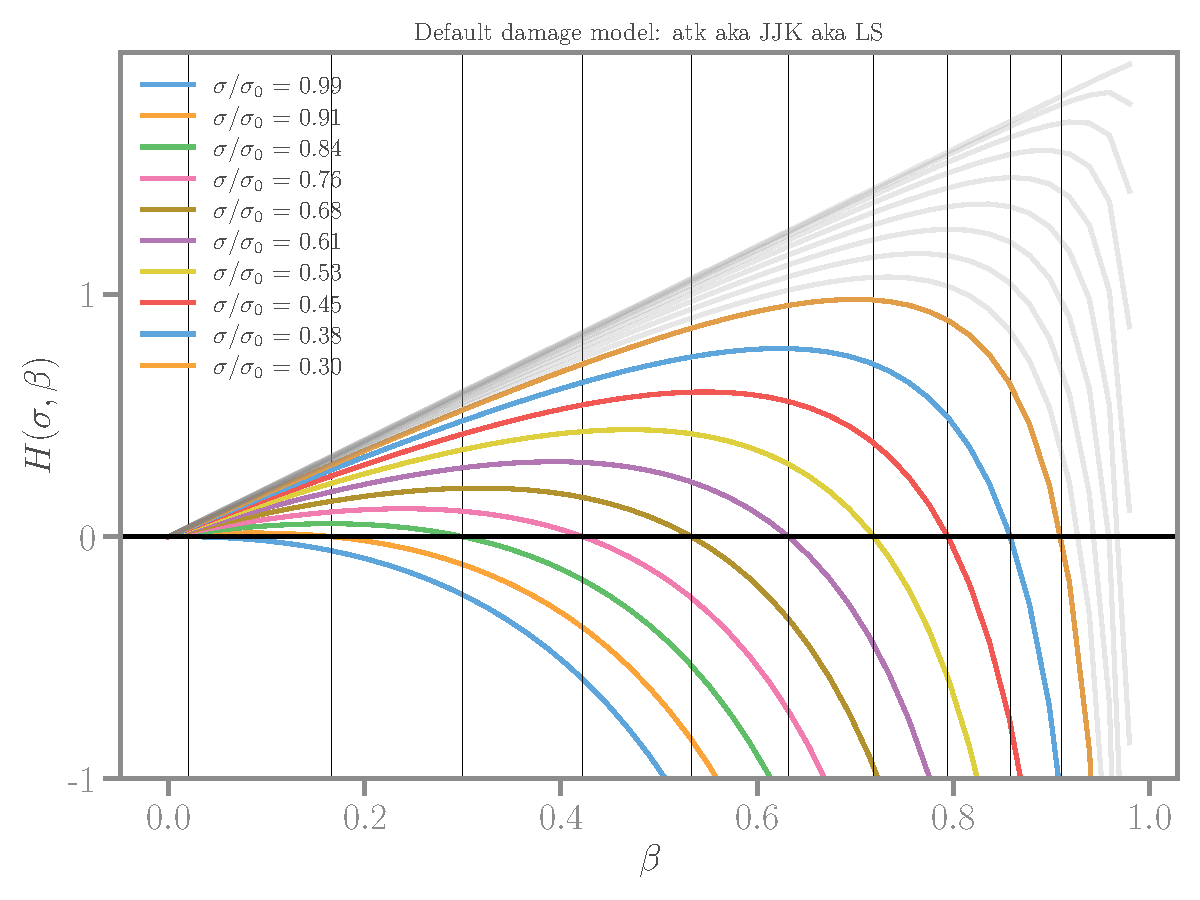
\includegraphics[width=.312\textheight, angle=90]{../figures/atk-Hbeta.pdf}
  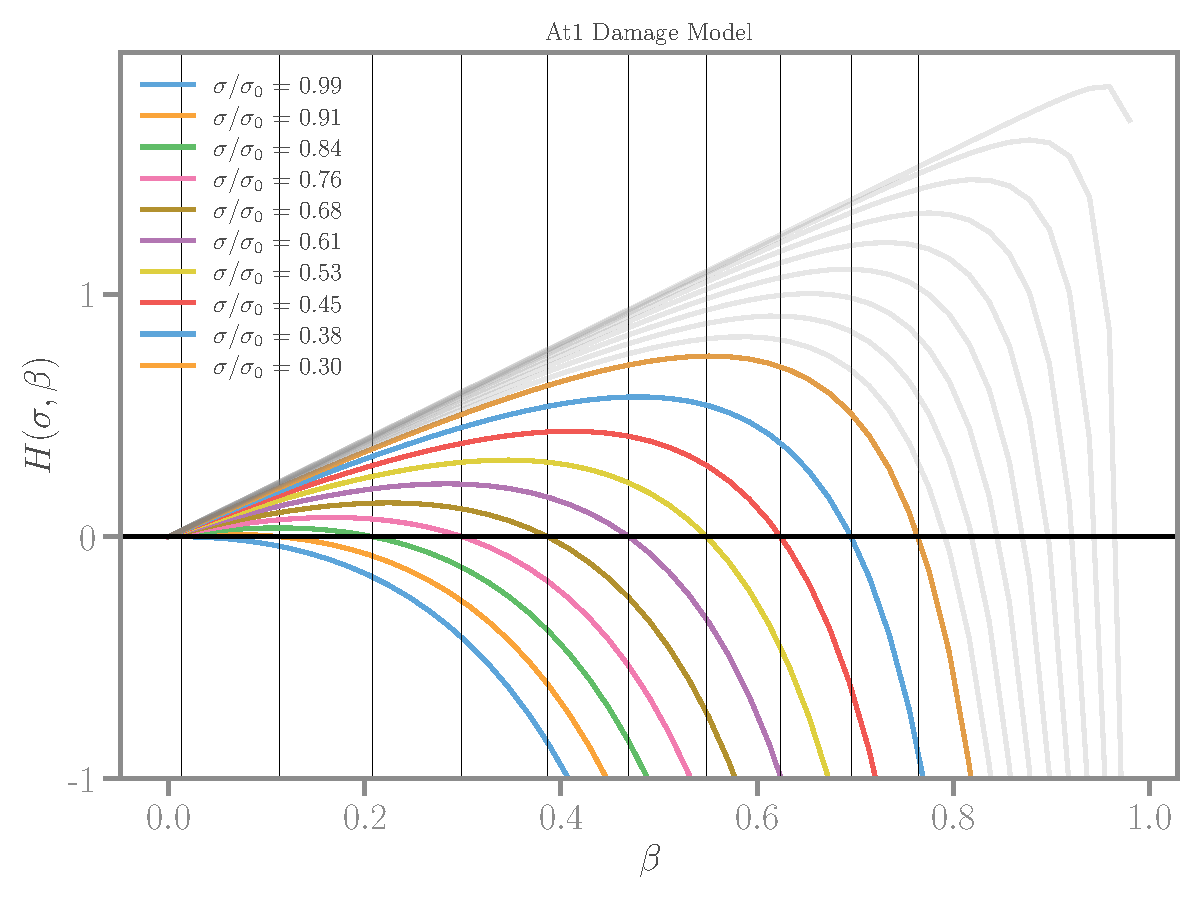
\includegraphics[width=.312\textheight, angle=90]{../figures/at1-Hbeta.pdf}
  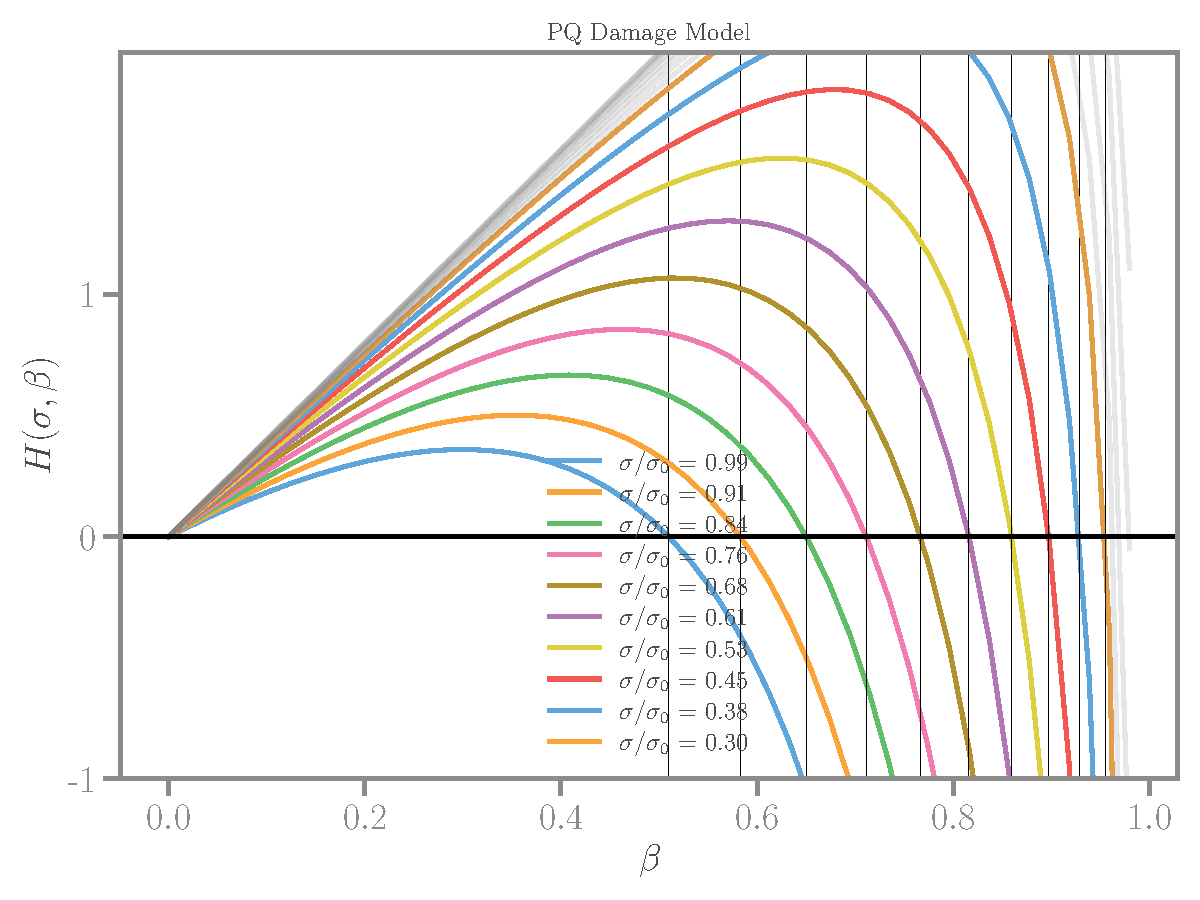
\includegraphics[width=.312\textheight, angle=90]{../figures/pq-Hbeta.pdf}
  \includegraphics[width=\textwidth]{../figures/Hprime-models.pdf}
  \caption{class analysis}
  \label{fig:class-analyser}
\end{figure}


\begin{figure}[htbp]
  \centering
  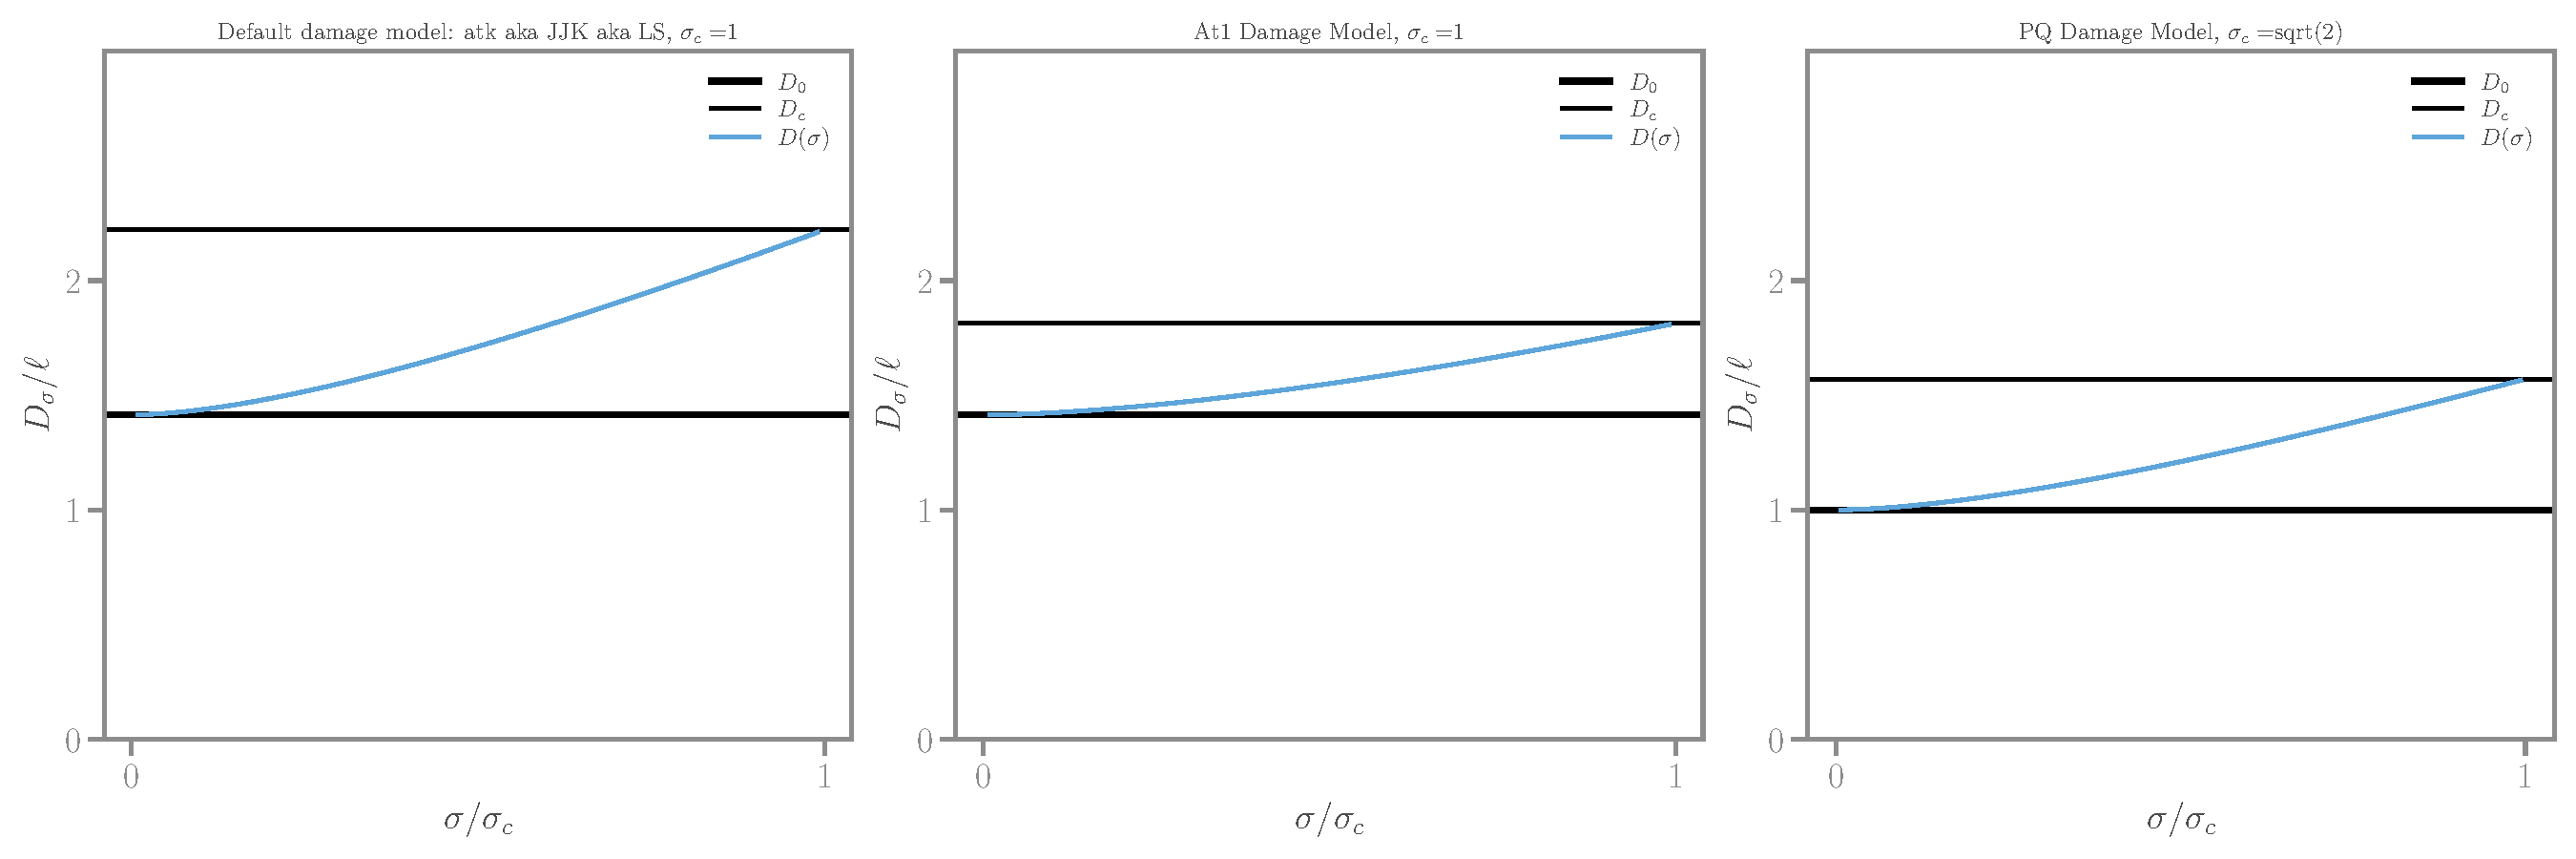
\includegraphics[width=\textwidth]{../figures/localisation-support-models.pdf}
  \caption{Halfsize of localisation support}
  \label{fig:support-analyser}
\end{figure}


\clearpage

\subsection*{Bifurcations}
How to \emph{successfully} integrate? 
$$ 
\int_0^{1} \frac{d \gamma}{\sqrt{H(\sigma, \alpha_0 \gamma)}} = \int_0^{1} \frac{d \gamma}{\sqrt{\bar H(\sigma,\gamma)}}
$$
La fonction $H$ s'annule en $\gamma=0, \gamma=\alpha_0$, ses dérivées étant bornées pour $\sigma>0$, 
$H'_\sigma(\gamma=1)$ est négative et explose, $H'_\sigma(\gamma=0)$ est positive.
L'integrale devrait converger, mais je n'arrive pas à le calculer numériquement, ni par integration symbolique, ni par quadrature.

Sebastien : saurais-tu integrer cette fonction numériquement? (ou symboliquement, avec Mathematica)
dans un des cas de figure des modeles ATk, AT1, PQ?
Puisque $H'(0), H'(1)$ sont bornés, la singularité devrait etre portée par un terme de la forme $({x-x_0})^{-1/2}$, integrable autour de $x_0$.

\begin{figure}[htbp]
  \begin{center}
  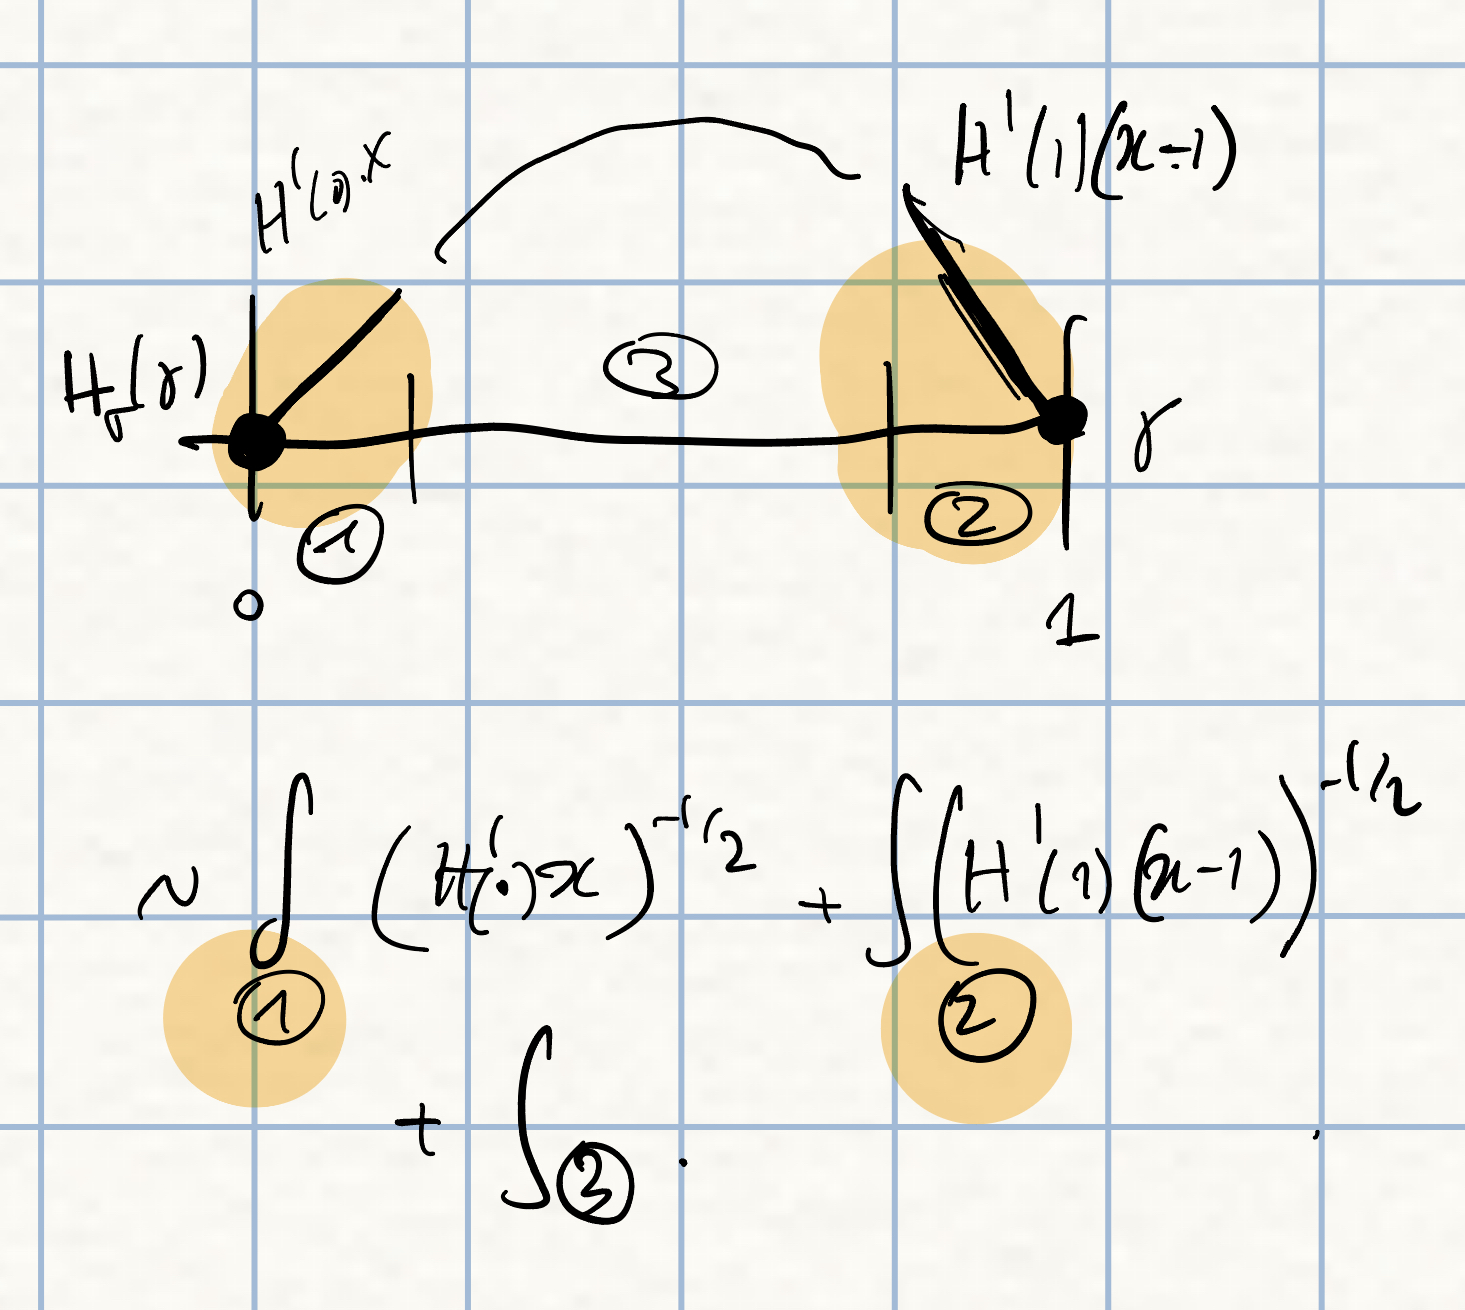
\includegraphics[width=.5\textwidth]{../figures/H-heuristics.jpeg}
  \caption{$H$ has two zeros. How to \emph{succesfully} integrate?}
  \label{fig:class-analyser}
  \end{center}
\end{figure}


\textbf{ATk}
\subimport{../../playground/nb/}{/H-atk.txt}
\begin{figure}[htbp]
  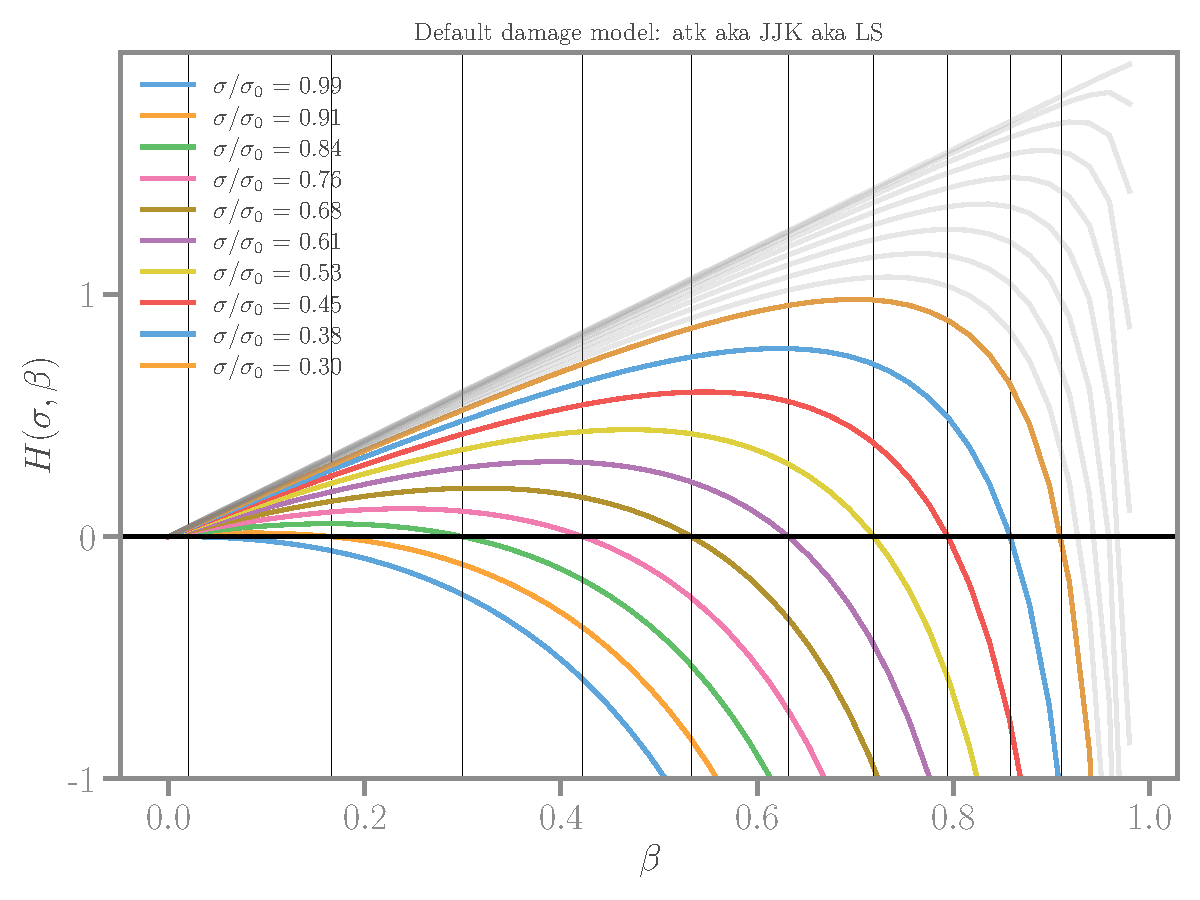
\includegraphics[width=.33\textheight]{../figures/atk-Hbeta.pdf}
  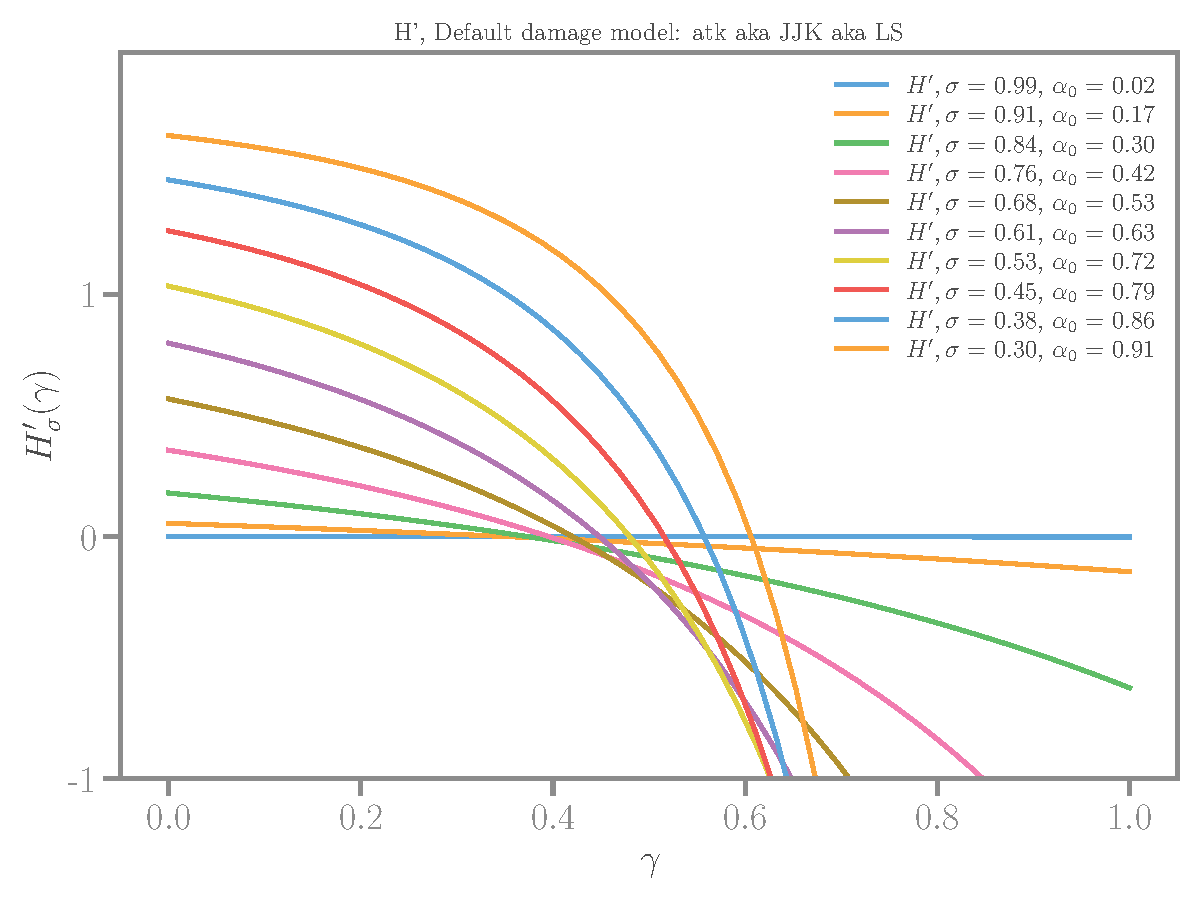
\includegraphics[width=.33\textheight]{../figures/atk-H-prime-beta.pdf}
  \caption{class analysis}
  \label{fig:class-analyser}
\end{figure}
\textbf{AT1}
\subimport{../../playground/nb/}{/H-at1.txt}
\begin{figure}[htbp]
  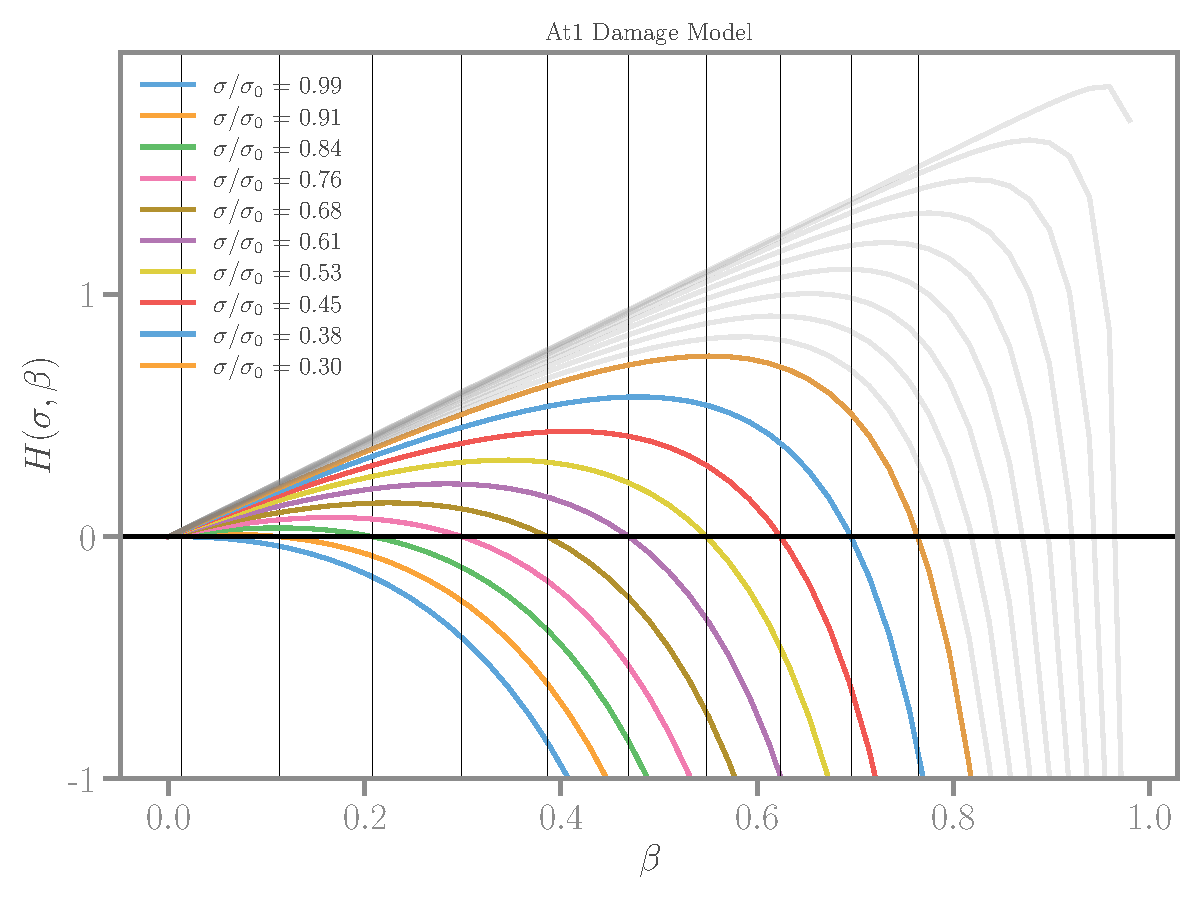
\includegraphics[width=.33\textheight]{../figures/at1-Hbeta.pdf}
  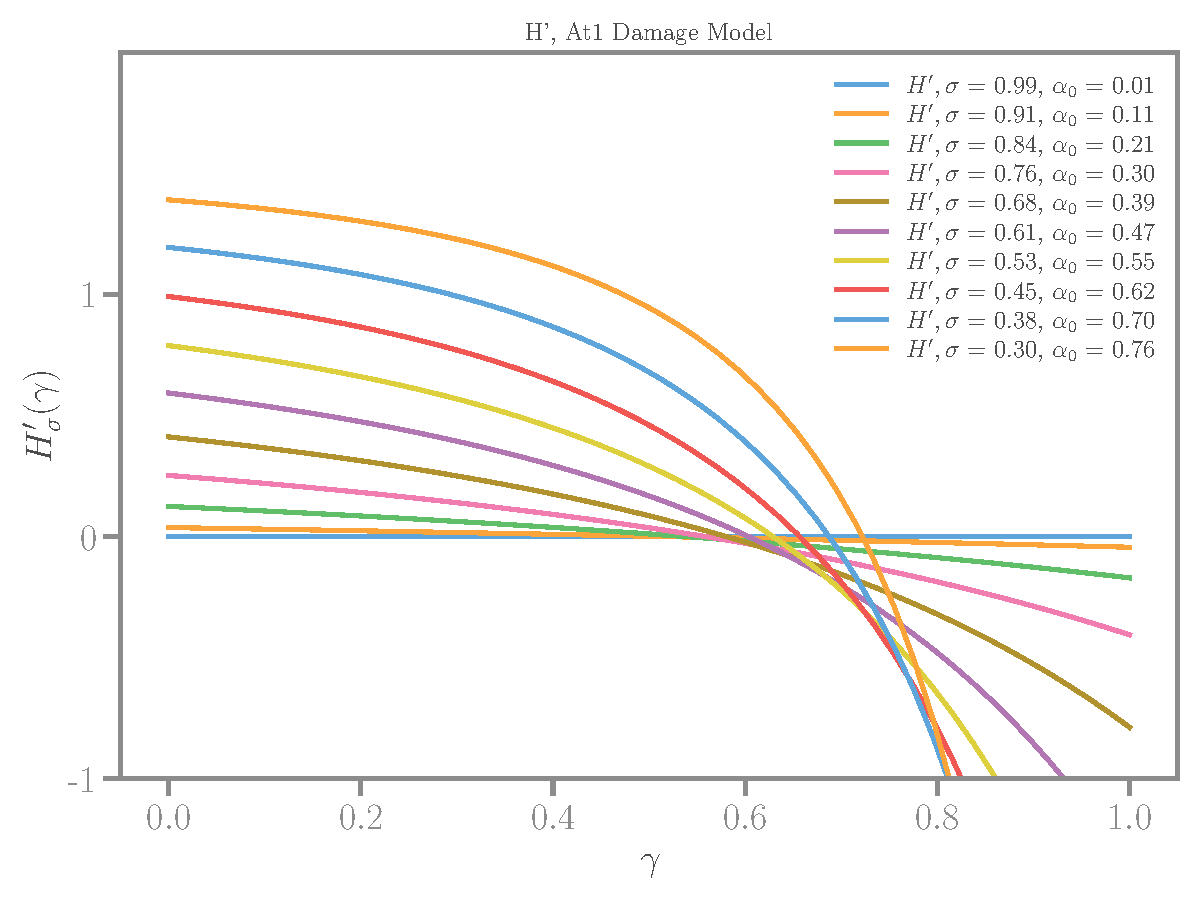
\includegraphics[width=.33\textheight]{../figures/at1-H-prime-beta.pdf}
  \caption{class analysis}
  \label{fig:class-analyser}
\end{figure}
\textbf{PQ}
\subimport{../../playground/nb/}{/H-pq.txt}
\begin{figure}[htbp]
  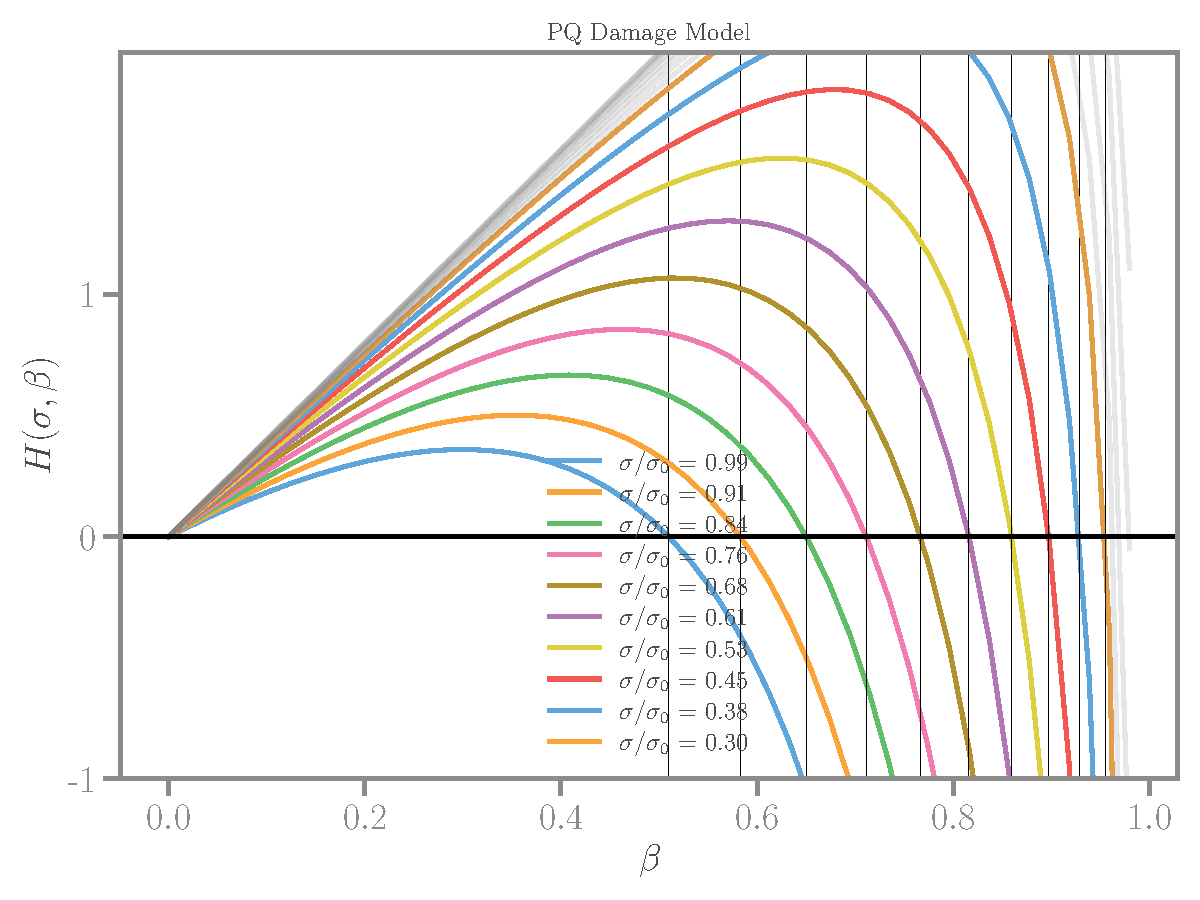
\includegraphics[width=.33\textheight]{../figures/pq-Hbeta.pdf}
  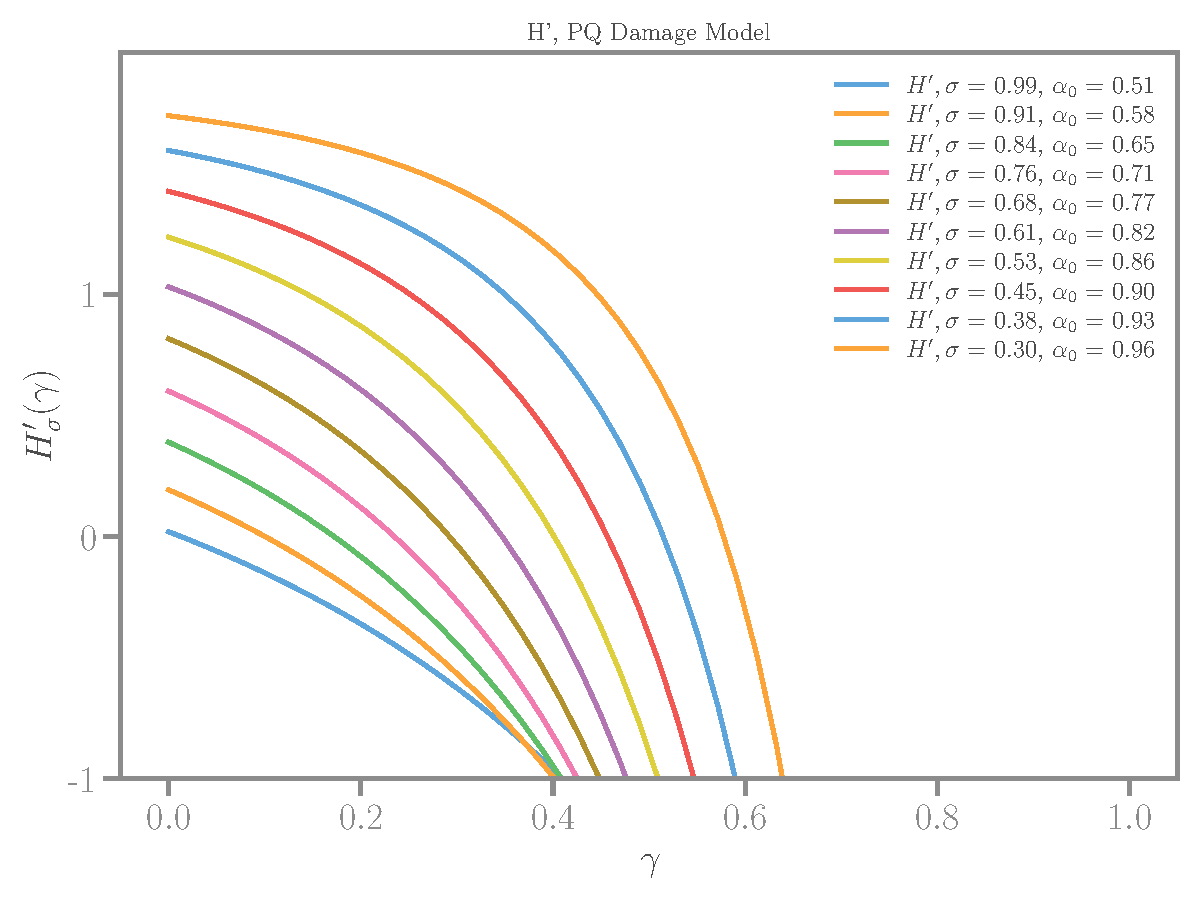
\includegraphics[width=.33\textheight]{../figures/pq-H-prime-beta.pdf}
  \caption{class analysis}
  \label{fig:class-analyser}
\end{figure}



\clearpage

\subsection*{Computations}
ATk
start from 

$$
\frac{2 \gamma \left(\sigma^{2} - 1\right) \left(\gamma \left(\sigma^{2} - 1\right) - \sigma^{2} + 1\right)}{- \gamma \left(\sigma^{2} - 1\right) - 1}
$$

substitute $\tau := \sigma^2 - 1$

\begin{equation}
  \label{eqn:}
  \frac{2 \gamma \tau^{2} \cdot \left(1 - \gamma\right)}{\gamma \tau + 1}
\end{equation}


..


To compute 

$$
D(\sigma):=\int_0^1( \bar H_\sigma(\gamma) )^{-1/2}\bar \alpha(\sigma) d \gamma
$$

ou $\beta = \bar \alpha \gamma$
$$
\bar H_\sigma(\gamma) := H(\sigma, \bar \alpha \gamma) 
$$

\end{document}

